\chapter{基于Zigzag映射矩阵的时间隐通道构建方法}
\label{chap:zigzag}

本章介绍的是基于Zigzag映射矩阵的时间隐通道构建方法,通过离散丢包的方式,丢弃具有特定数据包序号的数据包,实现隐蔽消息嵌入操作。由于RTP的数据包序号存在唯一性,发送方的主动丢包事件一定可以被接收方观测。接受方监听丢失的数据包序号,并根据鲁棒性方法去除噪声,便可得到隐蔽消息,完成时间隐通道的传输。基于Zigzag映射矩阵,实现了时间隐通道中码字到符号的映射,解除了码字与符号之间的线性关联。

%在下方加入各小节内容
\section{概述}
\label{chap:zigzag:overview}

根据时间隐通道的构建指标,时间隐通道应满足抗检测能力、鲁棒性、传输性能、构建代价及保密性方面的要求。VoLTE中基于主动丢包的时间隐通道,能够满足抗检测能力的约束,构建方法需要满足其余指标。因此在该构建方法中,通过结合Zigzag映射矩阵提高鲁棒性及保密性。

在鲁棒性方面,通过添加校验码字并结合Zigzag映射矩阵,将噪声影响离散化并通过验证校验实现去噪。借助CRC校验的确定性和随机性,调制过程中建立数据码字与校验码字的匹配关系,解调过程中通过重新验证校验关系区分噪声。

%该方法的创新点
该方法的创新点如下:
\begin{itemize}
	\item 提出了基于Zigzag映射矩阵的时间隐通道构建方法,并且具有足够的抗检测能力及鲁棒性;
	\item 基于Zigzag映射矩阵,建立了符号与码字之间的非线性映射;
	\item 引入了RTP中的随机字段,增加传输过程的随机化,增强隐蔽消息的保密性。
\end{itemize}

经实验验证,该时间隐通道在满足抗检测性的前提下,保证了一定的传输能力,满足了时间隐通道构建指标的要求。
\section{研究背景和动机}
\label{chap:zigzag:motivation}

本章主要介绍研究背景及研究动机,主要包括基于主动丢包的时间隐通道可行性分析,对Zigzag矩阵应用在码字-符号转换中的意义,及CRC校验如何提高时间隐通道的鲁棒性几个方面。结合\nref{chap:backinfo}对时间隐通道,及VoLTE视频通话场景的信道分析,参照\nref{chap:analyze}部分时间隐通道检测方法的测试,充分利用时间隐通道的构建基础,设计具有实际应用价值的构建方法,是本章的主要工作。

\subsection{基于主动丢包构建时间隐通道}
\label{chap:zigzag:motivation:dropout}
如图\nref{fig:2:pmf-dropout},VoLTE网络噪声中,长度为1的离散丢包占据总量的50\%左右。并且经过\nref{chap:analyze:result}实验的检验,当时间隐通道的主动丢包率降低到一定程度,即可规避现有的检测方法。因此,基于主动丢包的时间隐通道,在基本构造原理上依然可行。

对于隐通道的通信双方来说,如何有效识别数据包是一个非常重要的问题。在VoLTE中,可以有效利用RTP头中的Sequence Number字段,识别一次通话中数据包的唯一性。如图\nref{fig:2:rtp-header},数据包序号字段占据16 bit,最大可达到65536。正如\nref{chap:backinfo:rtp:dropout}对RTP丢包处理的描述,Sequence Number字段的作用,是识别一次通话中的数据包顺序,按照正确的顺序将负载提供给应用层。

基于数据包序号构建基于主动丢包的时间隐通道,具有以下优势:
\begin{itemize}
    \item 数据包序号具有传输同步能力,隐通道的传输过程以序号为参照时钟,无需时钟参照,简化了传输流程;
    \item 主动丢包行为不依赖数据包顺序,网络噪声中的乱序无法影响隐通道鲁棒性,防守方的数据包重排序也无法破坏隐通道;
    \item 防守方在防御时需要考虑对用户体验的影响,因此构造数据包填充丢包位置,对用户来说是可察觉的异常现象,一定程度上保证了丢包位置的传递;
    \item 如果防守反对数据包序号字段进行了覆写,则时间戳增长的线性关系被破坏,接收方可以监测到异常,并终止会话。
\end{itemize}

\subsection{ZigZag矩阵及其特征}
\label{chap:zigzag:motivation:zigzag}

\insertFigure{
	\begin{figure}
		\centering
        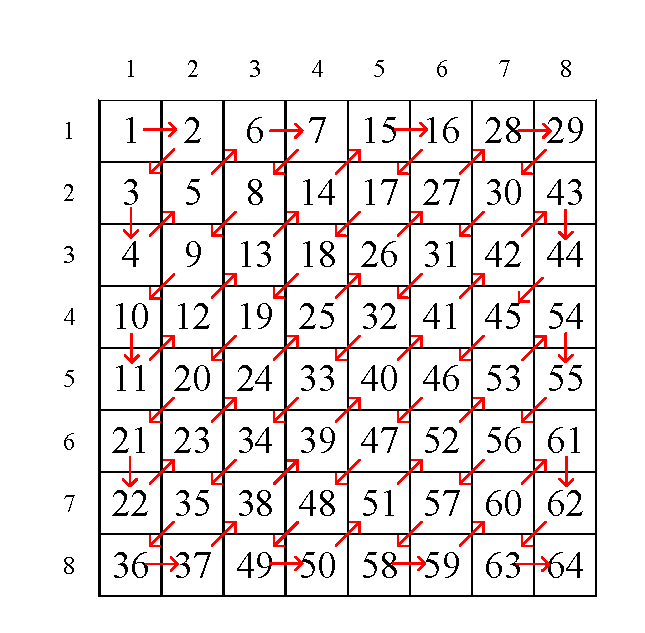
\includegraphics[width=0.6\textwidth]{chapters/chapter4/figures/zigzag-matrix.pdf}
        \caption{$8\times 8$的Zigzag矩阵示意图}
        \label{fig:4:zigzag-matrix}
	\end{figure}
}

Zigzag矩阵的排布方式,区别于常见的行优先或列优先,采用的是对角线折返的方式,不具备明显的线性关系。\nupcite{ji2015a,zaidee2006content,yang2018adaptive,li2019a}如图\nref{fig:4:zigzag-matrix}所示,矩阵中元素的坐标$(x,y)$,与元素的对应关系,由矩阵的规模决定。对于$L_{Codeword}=8$的时间隐通道来说,码字可以按照4 bit切分为上半部及下半部。参照Zigzag映射矩阵的定义,$(Codeword_{4~7},Codeword_{0~3})$可以对应到序号$Symbol$。

另一方面,Zigzag矩阵作为映射矩阵,其起始值支持用户设定,隐通道的双方可以约定一个安全的起始值,提高隐通道的保密性。即使防守方破解了隐通道的工作模式,并按照相同的解调方式,破解隐蔽消息,则需要对所有的可行解进行推测,提高了计算复杂度。随着矩阵规模的增大,矩阵中元素的排布关系会更加复杂,满足了隐通道的保密性要求。

\subsection{CRC数据校验策略}
\label{chap:zigzag:motivation:crc}

CRC是Cyclic Redundancy Check的缩写,全称为循环冗余校验码,在计算机网络及数据存储中有广泛应用。CRC作为散列函数的一种,可以生成数据的唯一摘要,根据位数的区别,常用的模式为CRC16及CRC32,更多的位数可以保证更低的冲突概率。在本时间隐通道中,CRC主要用于校验码字的正确性,无法使用全部的CRC校验值,因此,CRC16产生的结果可以基本满足校验的需求。

\insertFigure{
	\begin{figure}
		\centering
        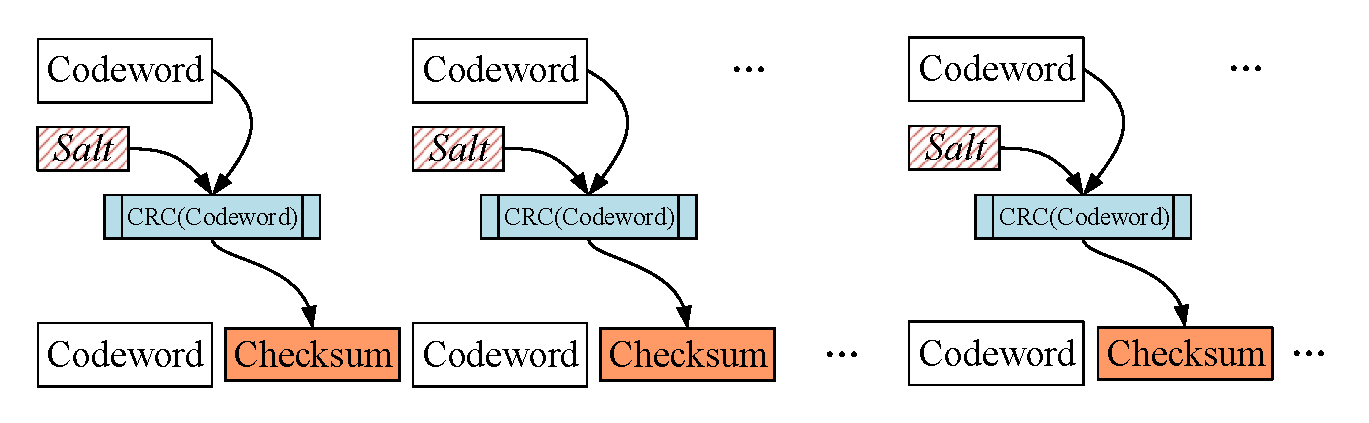
\includegraphics[width=0.98\textwidth]{chapters/chapter4/figures/insert-crc.pdf}
        \caption{CRC校验添加模式示意图}
        \label{fig:4:insert-crc}
	\end{figure}
}

如图\nref{fig:4:insert-crc},在每个数据码字之后,追加一个校验码字,通过校验码字区分噪声及信号。在CRC的参数方面,除了当前待验证的码字,额外引入$Salt$变量,增加计算结果的随机性及保密性。$salt$由两部分组成,一部分是用户自定义的私有值,一部分是RTP数据包头中导出的随机字段。在掺杂网络噪声的场景中,借助散列函数的单向性,提高防守方破解隐蔽消息的难度及计算量。

\insertTable{
	\begin{table}[]
      \centering
      \caption{添加CRC校验后的码字密度表}
      \label{tab:4:codeword-density}
          \begin{tabular*}{0.98\textwidth}{@{\extracolsep{\fill}}ccccc}
            \toprule
            $L_{Codeword}$ (bit) & 码字及校验长度 (bit) & 数据包数 & 校验编码利用率 & 总体编码利用率 \\
            \midrule
            6 & 12 & 128 & 65.6\% & 83.6\% \\
            7 & 14 & 256 & 66.4\% & 82.4\% \\
            8 & 16 & 512 & 68.0\% & 81.1\% \\
            9 & 18 & 1024 & 64.5\% & 82.2\% \\
            10 & 20 & 2048 & 62.8\% & 81.3\% \\
            11 & 22 & 4096 & 62.9\% & 81.9\% \\
            12 & 24 & 8192 & 63.2\% & 81.8\% \\
            \bottomrule
          \end{tabular*}
    \end{table}
}

通过组合码字及CRC校验信息,等价于形成了一个超长码字,并且码字中自带校验信息。采取数据及校验分别传输的方式,能够有效提高码字的传输效率,同时保证信道资源的利用率。如表\nref{tab:4:codeword-density},按照一个数据码字对应一个校验码字的方式,传输一个码字,需要$2^{L_{Codeword}}\times 2$个数据包才能完成调制。由于在有限位数限制下,CRC摘要的结果只能截取$L_{Codeword}$ bit,因此,在传输校验码字中存在无法利用的编码位置,因此校验部分的编码利用率在65\%左右,总体的编码利用率在82\%左右。

\subsection{研究动机}
\label{chap:zigzag:motivation:conclude}
通过主动丢包的方式构建时间隐通道,最直接的方式是对数据包范围进行分片,每片中丢弃一个数据包,以数据包的相对位置代表隐蔽消息中的数据。但这种传输模式,在网络噪声干扰的情况下,无法确保接收方能够准确接收到隐蔽消息。此外,时间隐通道传输传输的都是隐蔽的敏感信息,直接的传输模式无法保证隐蔽消息的安全性,即使消息自身已经加密。

\insertFigure{
	\begin{figure}
		\centering
        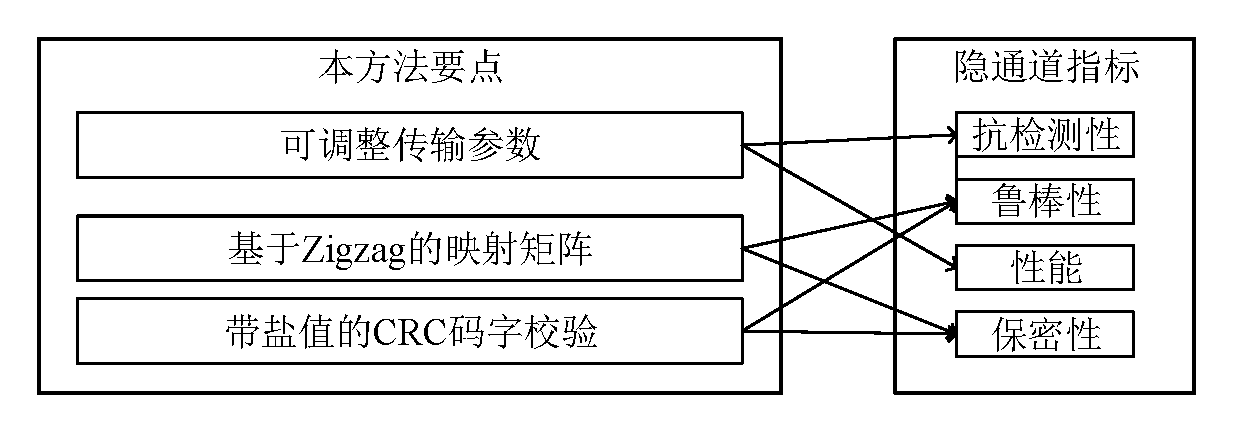
\includegraphics[width=0.8\textwidth]{chapters/chapter4/figures/method-struct.pdf}
        \caption{基于Zigzag映射矩阵的时间隐通道研究要点与指标}
        \label{fig:4:method-struct}
	\end{figure}
}

本章所研究的构建方法,在分片调制的基础上,对每个分片内所传输数据的内容进行调整,提高抗噪声干扰能力。如图\nref{fig:4:method-struct},在鲁棒性方面基于CRC校验,在传输数据码字的过程中穿插校验码字,通过校验信息进行有效数据筛选。在抗检测性方面,参数设置支持不同的$L_{Codeword}$,在Excellent场景与Good场景中对应配置。在保密性方面,引入Zigzag映射矩阵,在码字与符号之间添加一层转换,并且配合初始化参数实现映射矩阵的随机化;同时,在计算CRC校验值时,添加盐值增加结果的随机程度,提高反向破解难度。
\section{基于Zigzag映射矩阵的时间隐通道构建方法}
\label{chap:zigzag:model}

本节对构建方法进行详细介绍,包括设计架构、调制流程及解调流程三个部分。设计架构部分,主要介绍该时间隐通道的主要流程,设计的处理环节及数据对象。调制流程部分,主要介绍调制过程中的流程、计算方法及数据处理流程。解调流程部分,主要介绍解调过程中,如何根据丢包序号还原隐蔽消息,包括数据转换及数据检验等部分。

\subsection{设计架构}
\label{chap:zigzag:model:system}

\insertFigure{
	\begin{figure}[htbp]
		\centering
        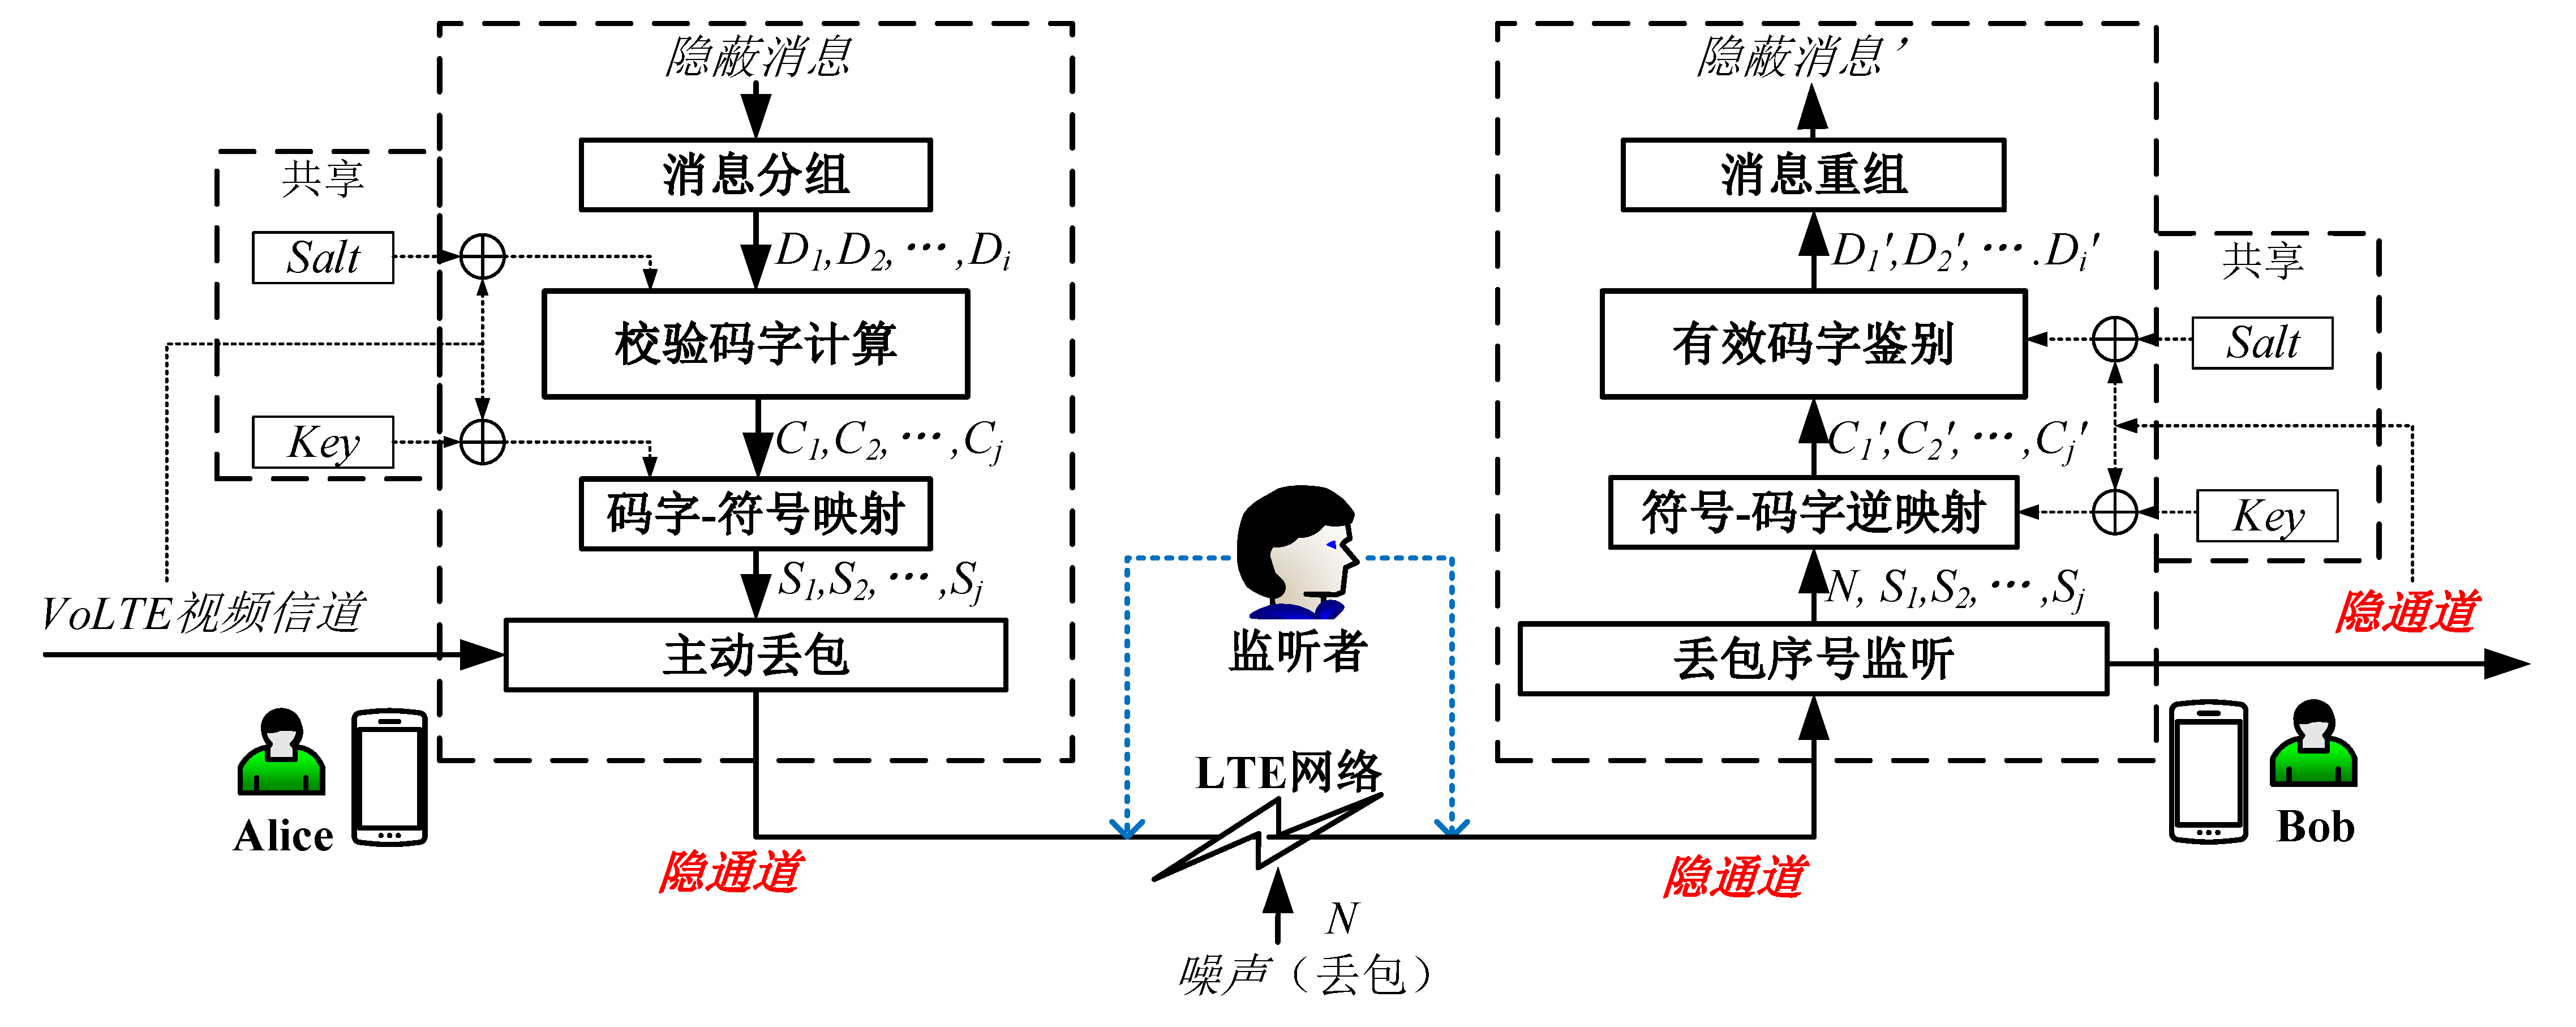
\includegraphics[width=0.98\textwidth]{chapters/chapter4/figures/system-model.pdf}
        \caption{基于Zigzag映射矩阵的时间隐通道系统模型图}
        \label{fig:4:system-model}
	\end{figure}
}

如图\nref{fig:4:system-model},对于用户Alice和Bob,希望通过该时间隐通道传输隐蔽消息,而监听者对两人的所有通信进行了监听,只允许进行被监听的VoLTE通话。在进行传输前,接收方与发送方预先约定一个私有的$Key$及$Salt$,类似消息加密的私有秘钥,用于CRC校验生成及映射矩阵初始化。调制过程的消息分组阶段,完成对隐蔽消息的分组,生成定长的消息块$D_{i}$。校验码字计算阶段依赖CRC算法,结合私有$Salt$及宿主信道中提取的随机信息,计算每个码字的校验值,生成所有码字$C_{j}$。码字-符号映射阶段,利用私有$Key$及随机信息初始化映射矩阵,将码字$C_{j}$映射到相对序号$S_{j}$。主动丢包阶段,监控当前的数据包传输状态,并将目标数据包直接丢弃。

VoLTE数据包经LTE网络传输后,时间隐通道与网络噪声叠加。接收方监听到达的RTP数据包序号,并记录下丢失数据包的序号。按照调制过程的逆序,解调过程识别获取的符号$S_{j}^{'}$,然后参照逆映射矩阵将符号$S_{j}^{'}$转换为码字$C_{j}^{'}$,逆映射时映射矩阵的初始化参数与调制阶段保持一致。有效码字鉴别阶段根据CRC校验码字,筛选出符合校验规则的数据块$D_{i}^{'}$。最终消息重组阶段组合所有的消息块,得到隐蔽消息。

\subsection{调制流程}
\label{chap:zigzag:model:modulation}

\insertFigure{
	\begin{figure}[htb]
		\centering
        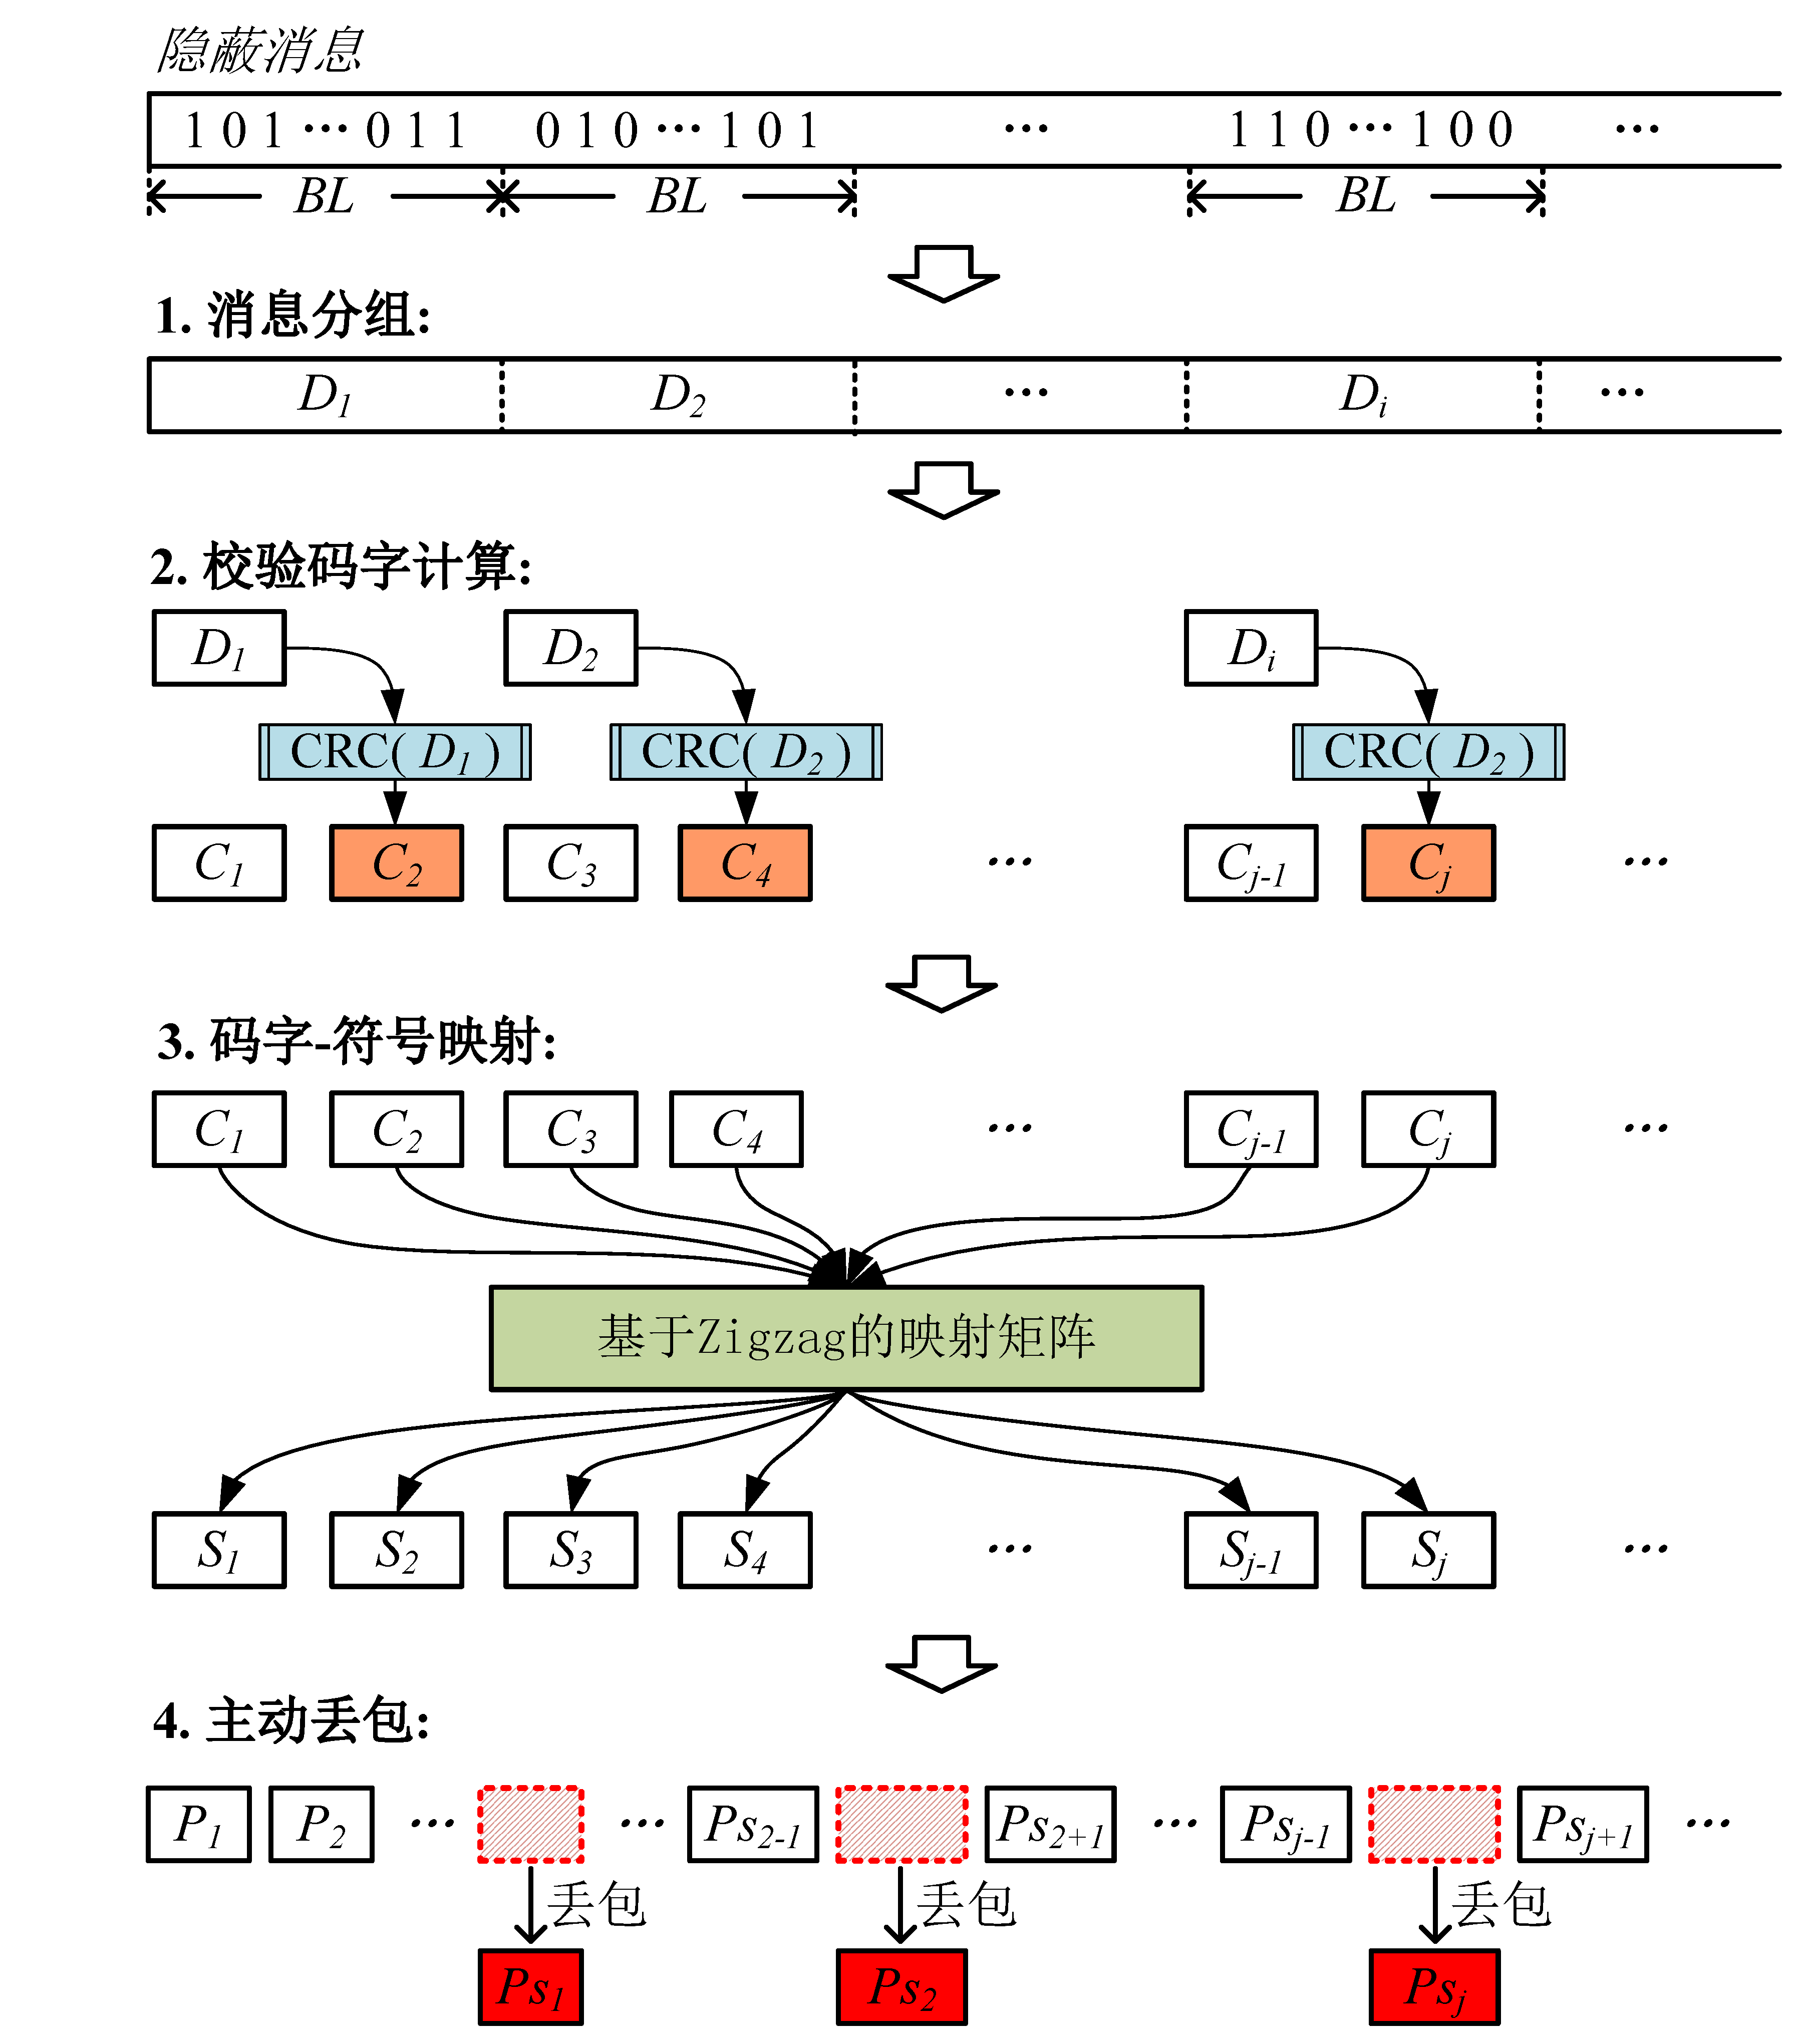
\includegraphics[width=0.8\textwidth]{chapters/chapter4/figures/modulation-flow.pdf}
        \caption{基于Zigzag映射矩阵的时间隐通道调制流程}
        \label{fig:4:modulation-flow}
	\end{figure}
}

如图\nref{fig:4:modulation-flow},调制过程中的处理步骤可以分为四个阶段,与系统模型中的各阶段对应。待发送的隐蔽消息为输入变量,最终结果为具有序号$S_{j}$的数据包被丢弃。

\subsubsection{隐蔽消息分组}
\label{chap:zigzag:model:modulation:segment}
隐蔽消息按照参数$BL$,切分为定长的消息块$D_{i}$,每个消息块单独调制。相对丢包位置与消息块长度匹配,则传输每个符号需要的数据包数量为$2^{BL}$。对于本方法,码字中没有额外的校验信息,因此$L_{Codeword}=BL$。

\insertEquation{
    \begin{equation}
    \label{equ:4:throughput}
    \begin{split}
        Throughput\ &=\ \frac{L_{Codeword}}{2^{L_{Codeword}}}\ \times\ 100\quad (bps)\ \\
        &=\ \frac{BL}{2^{BL}}\ \times\ 100\quad (bps)
    \end{split}
    \end{equation}
}

当确定了传输参数$L_{Codeword}$,则该时间隐通道的传输性能可以通过公式(\nref{equ:4:throughput})计算,VoLTE视频数据包传输速率按照平均值$100\ (pkts/s)$计算。在有限的通话时间中,数据包总量是有限的,时间隐通道必须提高传输效率。在分组传输模式下,通信双方不需要同步时钟,提高了资源利用率。

\subsubsection{基于CRC的码字校验}
\label{chap:zigzag:model:modulation:crc}

计算CRC校验,需要结合用户自定义的私有$Salt$,以及由RTP传输流中导出的随机字段。在这里,选择RTP包头中的$SSRC$,与$Salt$进行异或后与消息块$D_{i}$进行拼接,共同作为CRC函数的参数。计算过程的描述如算法\nref{alg:4:codeword-generation},输入参数包括隐蔽消息及参数,最终返回生成的码字序列$C$。

\insertContents{
    \begin{algorithm}[htbp]
        \renewcommand{\algorithmcfname}{算法}
        \caption{码字生成}
        \label{alg:4:codeword-generation}
        \LinesNumbered
        \KwIn{$Covert\ Message,\ SSRC,\ Salt,\ L_{Codeword}$}
        \KwOut{$C\ \leftarrow\ \{\}$}
        $D\ \leftarrow\ \{\},\ offset\ \leftarrow\ 0$ \\
        \For {$offset\ <\ length(Covert\ Message)$} {
            $D_{i}\ \leftarrow\ Covert\ Message[offset\ :\ L_{Codeword}]$ \\
            append $\ D_{i}\ $ to $\ D$
        }
        $salt\ \leftarrow\ Salt\ \oplus\ SSRC$ \\
        \For {$D_i\ $ in $\ D$} {
            $C_{j}\ \leftarrow\ $CRC16\ ($salt\ //\ D_{i}\ //\ salt$) \\
            append $\ D_{i}\ $ to $\ C_{j}$ \\
            append $\ C_{j}\ $ to $\ C$
        }
        \Return $C$
    \end{algorithm}
}

\subsubsection{基于Zigzag的映射矩阵}
\label{chap:zigzag:model:modulation:mapping}

映射矩阵实现了码字$C_{j}$到符号$S_{j}$的转换,矩阵中元素数量由$L_{Codeword}$决定。矩阵的行数与列数如公式(\nref{equ:4:matrix-length})计算,映射矩阵$\textit{\textbf{M}}$为方阵,且满足$M_{cols}\times M_{rows}=2^{L_{Codeword}}$。映射矩阵的映射关系,是本方法保密性的重要环节。图\nref{fig:4:zigzag-matrix}中$M_{1,\ 1}$由1开始排布,而实际应用中,$M_{1,\ 1}$由用户设定的$Key$及RTP中的随机字段决定,计算公式如公式(\nref{equ:4:matrix-begin})。映射矩阵排布完毕后,对每个元素$\textit{\textbf{M}}_{i,\ j}$取模,确保不超过上限$2^{L_{Codeword}}$。

\insertEquation{
    \begin{equation}
    \label{equ:4:matrix-length}
		M_{cols}\ =\ M_{rows}\ =\ 2^{\frac{L_{Codeword}}{2}}
    \end{equation}
    \begin{equation}
    \label{equ:4:mapping}
        S_{j}\ =\ \textit{\textbf{M}}_{C_{j,\ \lbrack L_{Codeword}/2,\ L_{Codeword})},\ C_{j,\ \lbrack 0,\ L_{Codeword}/2)}}
    \end{equation}
    \begin{equation}
    \label{equ:4:matrix-begin}
    \textit{\textbf{M}}_{1,\ 1}\ =\ (Key\ \oplus\ SSRC)\ \%\ 2^{L_{Codeword}}\ +\ 1
    \end{equation}
}

码字转换为符号的过程,由映射矩阵实现。对于码字$C_{j}$,其整体长度为$L_{Codeword}$\ bits,按照$L_{Codeword}/2$\ bits进行划分,得到前半部分$C_{j,\ [0,\ L_{Codeword}/2)}$,以及后半部分$C_{j,\ [L_{Codeword}/2,\ L_{Codeword})}$。参照图\nref{fig:4:zigzag-matrix}及映射矩阵实现,按照公式(\nref{equ:4:mapping})完成转换。

\subsection{解调流程}
\label{chap:zigzag:model:demodulation}

\insertFigure{
	\begin{figure}[htb]
		\centering
        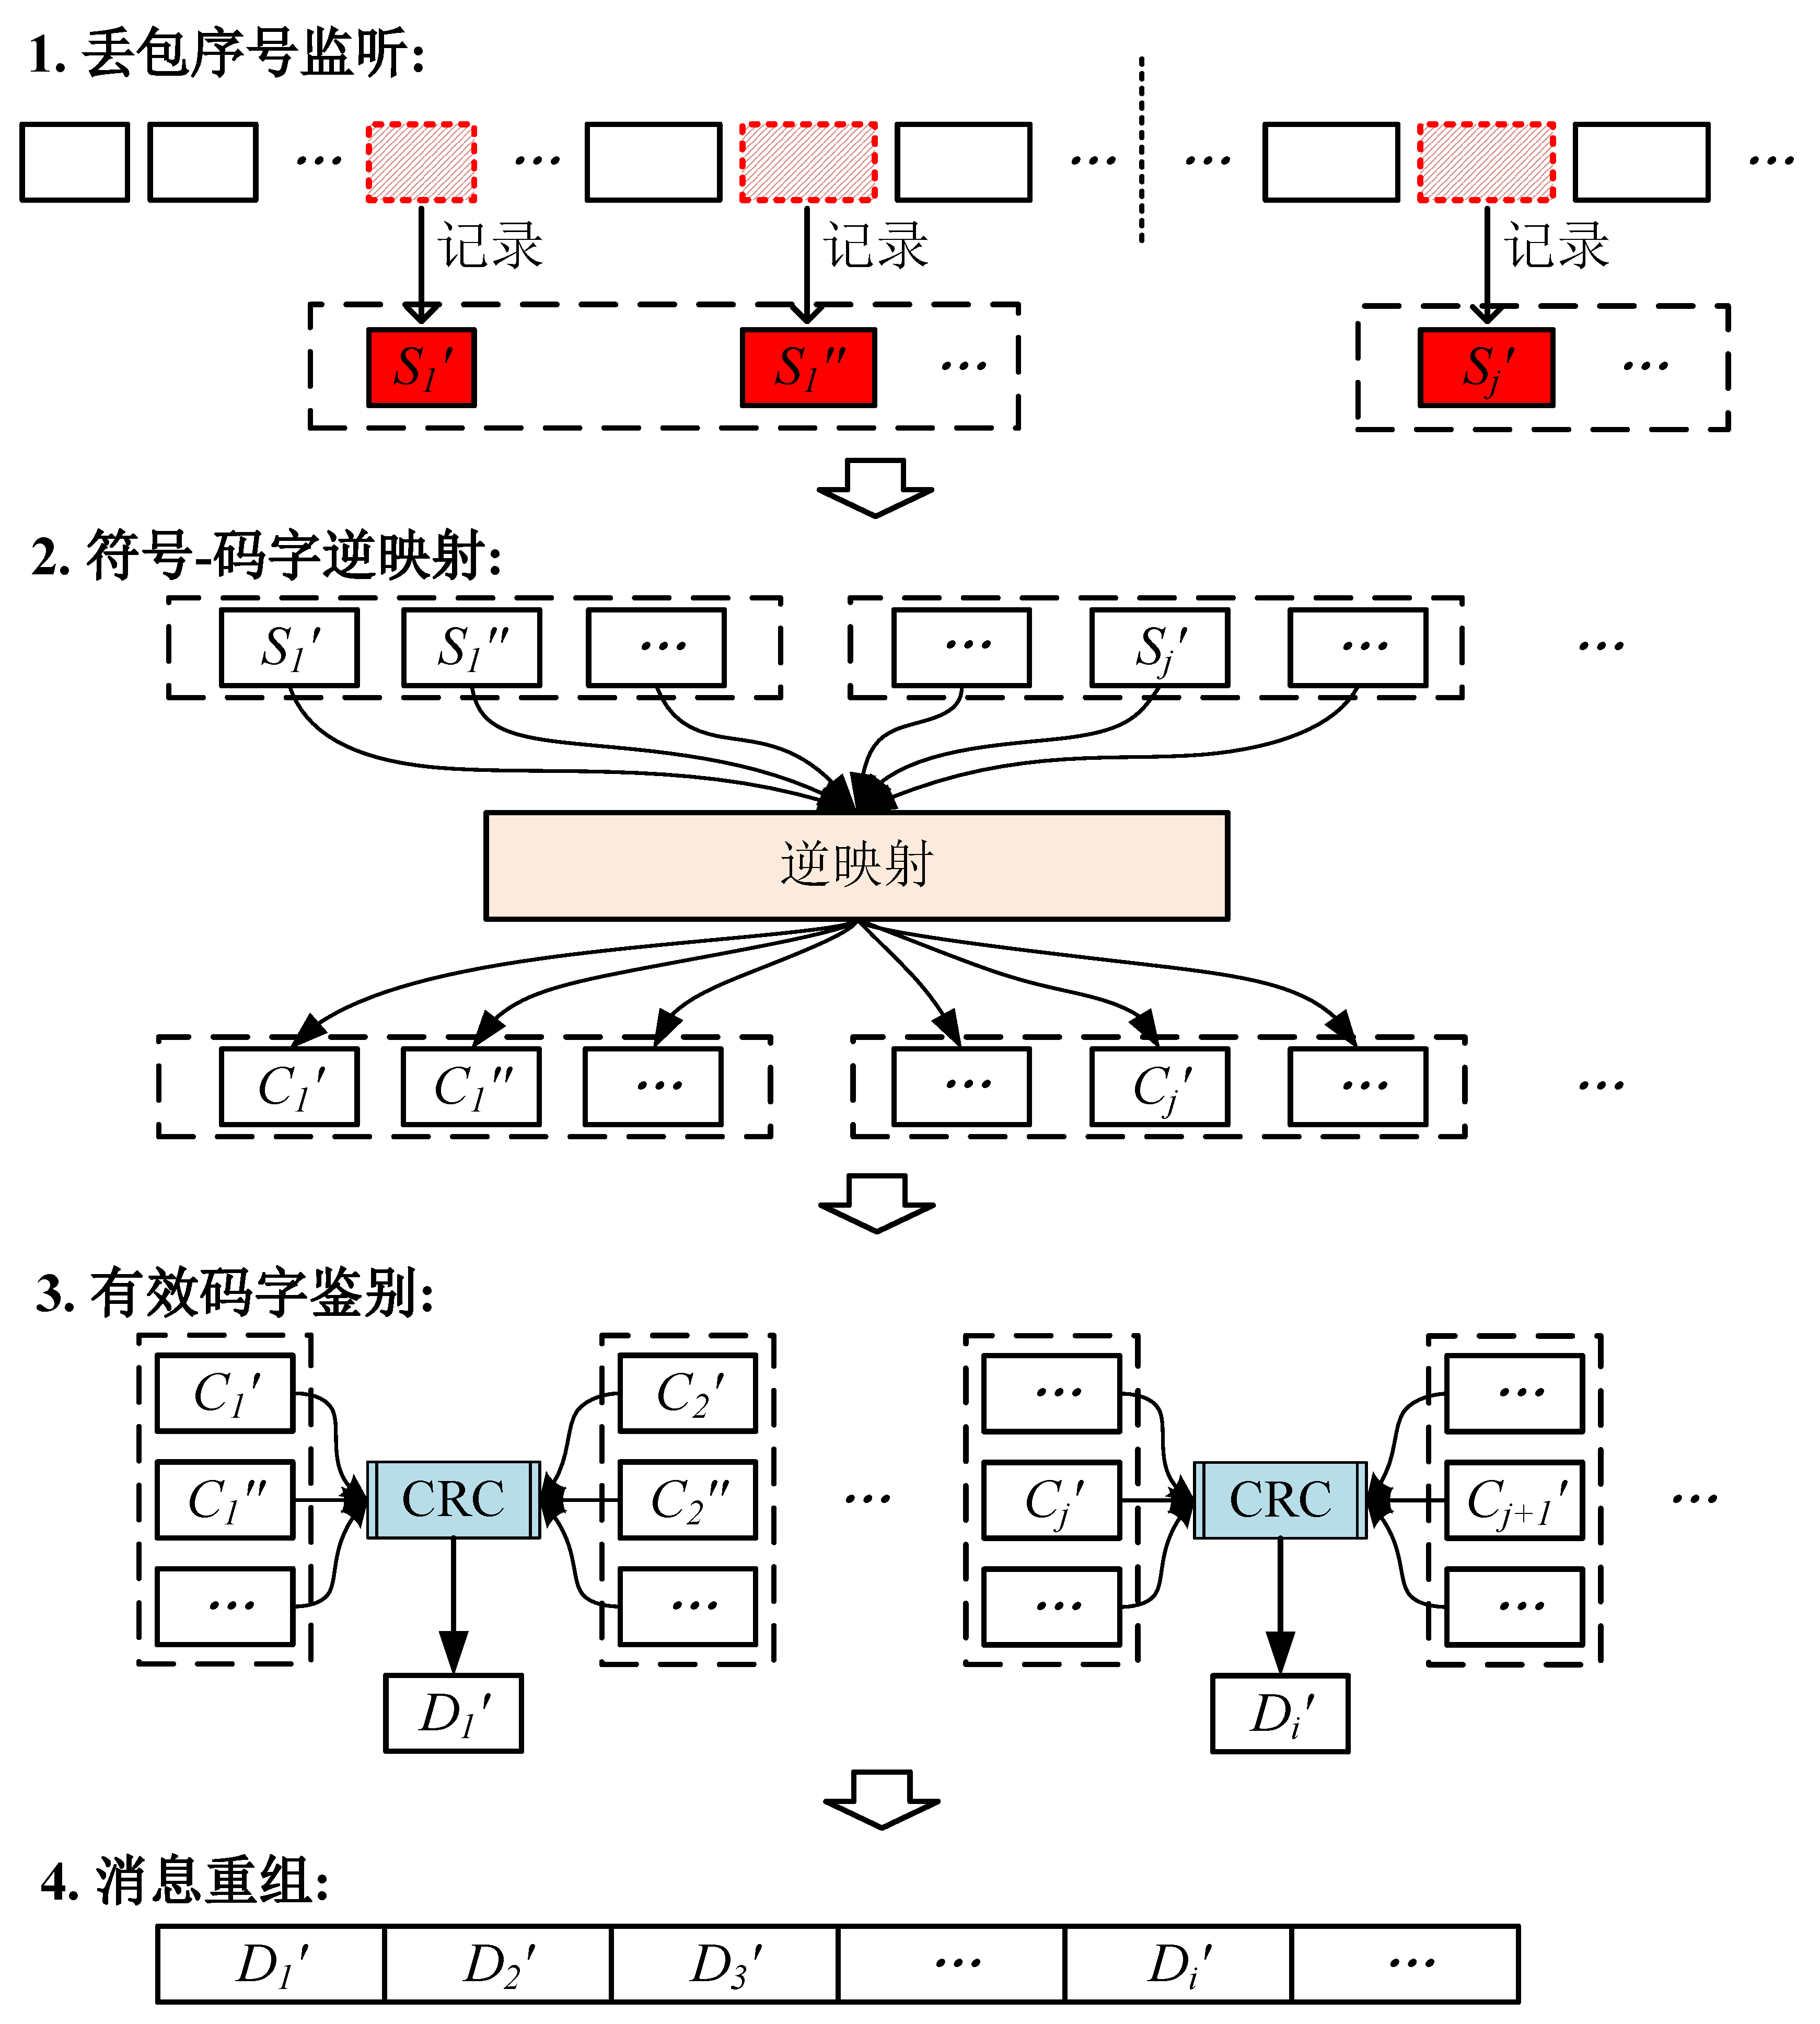
\includegraphics[width=0.8\textwidth]{chapters/chapter4/figures/demodulation-flow.pdf}
        \caption{基于Zigzag映射矩阵的时间隐通道解调流程}
        \label{fig:4:demodulation-flow}
	\end{figure}
}

如图\nref{fig:4:demodulation-flow},解调流程主要分为四个部分,分别为监听丢包序号、符号-码字逆映射、鉴别有效码字,以及消息重组。由于网络噪声不可避免,解调过程中每组的候选项不唯一,在完成验证前,所有的候选项都视为可行解。

\insertEquation{
    \begin{equation}
    \label{equ:4:group-id}
		j\ =\ \left \lfloor\frac{number\ -\ 1}{2^{L_{Codeword}}}\right \rfloor\ +\ 1
    \end{equation}
    \begin{equation}
    \label{equ:4:symbol}
        S_{j}\ =\ (number\ -\ 1)\ \%\ (2^{L_{Codeword}})\ +\ 1
    \end{equation}
}

根据映射矩阵的规模,每个矩阵对应的数据包数量为$2^{L_{Codeword}}$,则丢包序号$number$与$j$及$S_{j}$的对应关系如公式(\nref{equ:4:group-id})及公式(\nref{equ:4:symbol})。

\subsubsection{基于Zigzag矩阵的逆映射}
\label{chap:zigzag:model:demodulation:reverse-mapping}

映射矩阵将码字映射为符号,逆映射过程需要按照相同的规则还原码字。对于接收方来说,通过映射矩阵进行逆映射效率较低,需要首先生成映射矩阵的逆映射关系。按照调制过程相同的方式,在构建映射矩阵的过程中,创建逆映射关系$S_{j}\ \rightarrow\ C_{j}$,通过索引快速完成逆映射。

\subsubsection{有效码字鉴别}
\label{chap:zigzag:model:demodulation:identification}

\insertContents{
    \begin{algorithm}[htbp]
        \renewcommand{\algorithmcfname}{算法}
        \caption{有效码字鉴别}
        \label{alg:4:codeword-identification}
        \LinesNumbered
        \KwIn{$\{\{C_{1}',\ \cdots\},\ \{C_{2}',\ \cdots\},\ \cdots\},\ Salt,\ SSRC$}
        \KwOut{$D\ \leftarrow\ \{\}$}
        $salt\ \leftarrow\ Salt\ \oplus\ SSRC$ \\
        \For {$\{C_{j}',\ \cdots\},\ \{C_{j+1}',\ \cdots\}\ $ in $\ C$} {
            \For {$C_{j}'\ $ in $\ \{C_{j}',\ \cdots\}$} {
                $checksum\ =\ $CRC16\ ($salt\ //\ C_{j}'\ //\ salt$) \\
                \If {$checksum\ $ in $\ \{C_{j+1}',\ \cdots\}$} {
                    append $\ C_{j}'\ $ to $\ D$ \\
                    \textbf{break}
                }
            }
        }
        \Return $D$
    \end{algorithm}
}

在调制过程中,码字规模$j$是数据块规模$i$的2倍,即$j\ =\ 2\ \times\ i$。因此,解调过程中,可以划分为两部分,分别为奇数组的数据码字及偶数组的校验码字。如图\nref{fig:4:demodulation-flow},鉴别码字的过程中,重新计算校验值,判断校验值是否在校验码字中出现,即可判断当前数据码字的有效性。

码字鉴别过程的描述如算法\nref{alg:4:codeword-identification},首先计算盐值$salt$,同样由用户自定义的盐值$Salt$及随机字段$SSRC$组成。重新计算$C_{j}'$对应的校验码字,如果结果在$\{C_{j+1}',\ \cdots\}$中出现,则意味着$C_{j}'$符合校验规则。最终,组合所有的数据块$D_{i}'$,还原出隐蔽消息,解调过程结束。
\section{隐通道评估}
\label{chap:zigzag:results}
本节对基于Zigzag映射矩阵的时间隐通道进行评估,参照时间隐通道构建指标,评估由抗检测能力、鲁棒性、传输性能及构建代价四个方面组成。其中,抗检测能力测试按照本文\ \nref{chap:analyze:statistical}中提出的方法进行。

\subsection{评估环境及参数}
\label{chap:zigzag:results:environment}
该方法中,主要的参数为$L_{Codeword}$,其取值决定了传输性能,并对抗检测能力有影响。评估测试的场景,包括本文\ \nref{chap:analyze:results}中表\ \nref{tab:3:capture-results}对应的抓包结果,以及随机生成的网络噪声。

\insertTable{
	\begin{table}[htbp]
      \centering
      \caption{测试环境信息表}
      \label{tab:4:result:environment}
          \begin{tabular*}{0.9\textwidth}{@{\extracolsep{\fill}}cl}
            \toprule
            类型 & 详细信息 \\
            \midrule
            PC平台 & i5-9400,DDR4 16GB \\
            软件版本 & Windows 7,QT 5.9.5,python 3.6;Ubuntu 16.04,mysql 5.7 \\
            数据集 & VoLTE抓包结果,随机噪声 \\
            \bottomrule
          \end{tabular*}
    \end{table}
}

评估实验的软硬件环境如表\ \nref{tab:4:result:environment},所有的数据均存储到mysql数据库中,通过基于QT的时间隐通道处理逻辑,得到调制与解调结果。根据调制解调结果,评估抗检测能力等指标。基于python脚本,将抓包结果还原为视频数据,并评估调制前后的视频质量,得到隐通道构建代价测试结果。此外,为有效评估鲁棒性、比较不同丢包率下的误码率水平,生成了丢包率为0.5\ \%、1\ \%、2\ \%、5\ \%及10\ \%的五种随机噪声。

\insertTable{
	\begin{table}[htbp]
      \centering
      \caption{基于Zigzag映射矩阵时间隐通道的参数}
      \label{tab:4:parameters}
          \begin{tabular*}{0.5\textwidth}{@{\extracolsep{\fill}}ccc}
            \toprule
            $L_{Codeword}$\ (bits) & $2^{L_{Codeword}}$ & 主动丢包率 \\
            \midrule
            7 & 128 & 0.781\ \% \\ 
            8 & 256 & 0.391\ \% \\ 
            9 & 512 & 0.195\ \% \\ 
            10 & 1024 & 0.098\ \% \\ 
            11 & 2048 & 0.049\ \% \\ 
            \bottomrule
          \end{tabular*}
    \end{table}
}

参照本文\ \nref{chap:analyze:result}的实验结果,参数$L_{Codeword}$的取值如表\ \nref{tab:4:parameters},在具备抗检测能力的前提下,进行其它指标的测试。

\subsection{抗检测能力测试}
\label{chap:zigzag:results:undetectability}

\subsubsection{IPD检测}
\label{chap:zigzag:results:undetectability:ipd}

\insertFigure{
	\begin{figure}[htbp]
        \centering
        \subfigure[Excellent场景的CDF曲线]{
            \label{fig:4:results:ipd:cdf:excellent}
            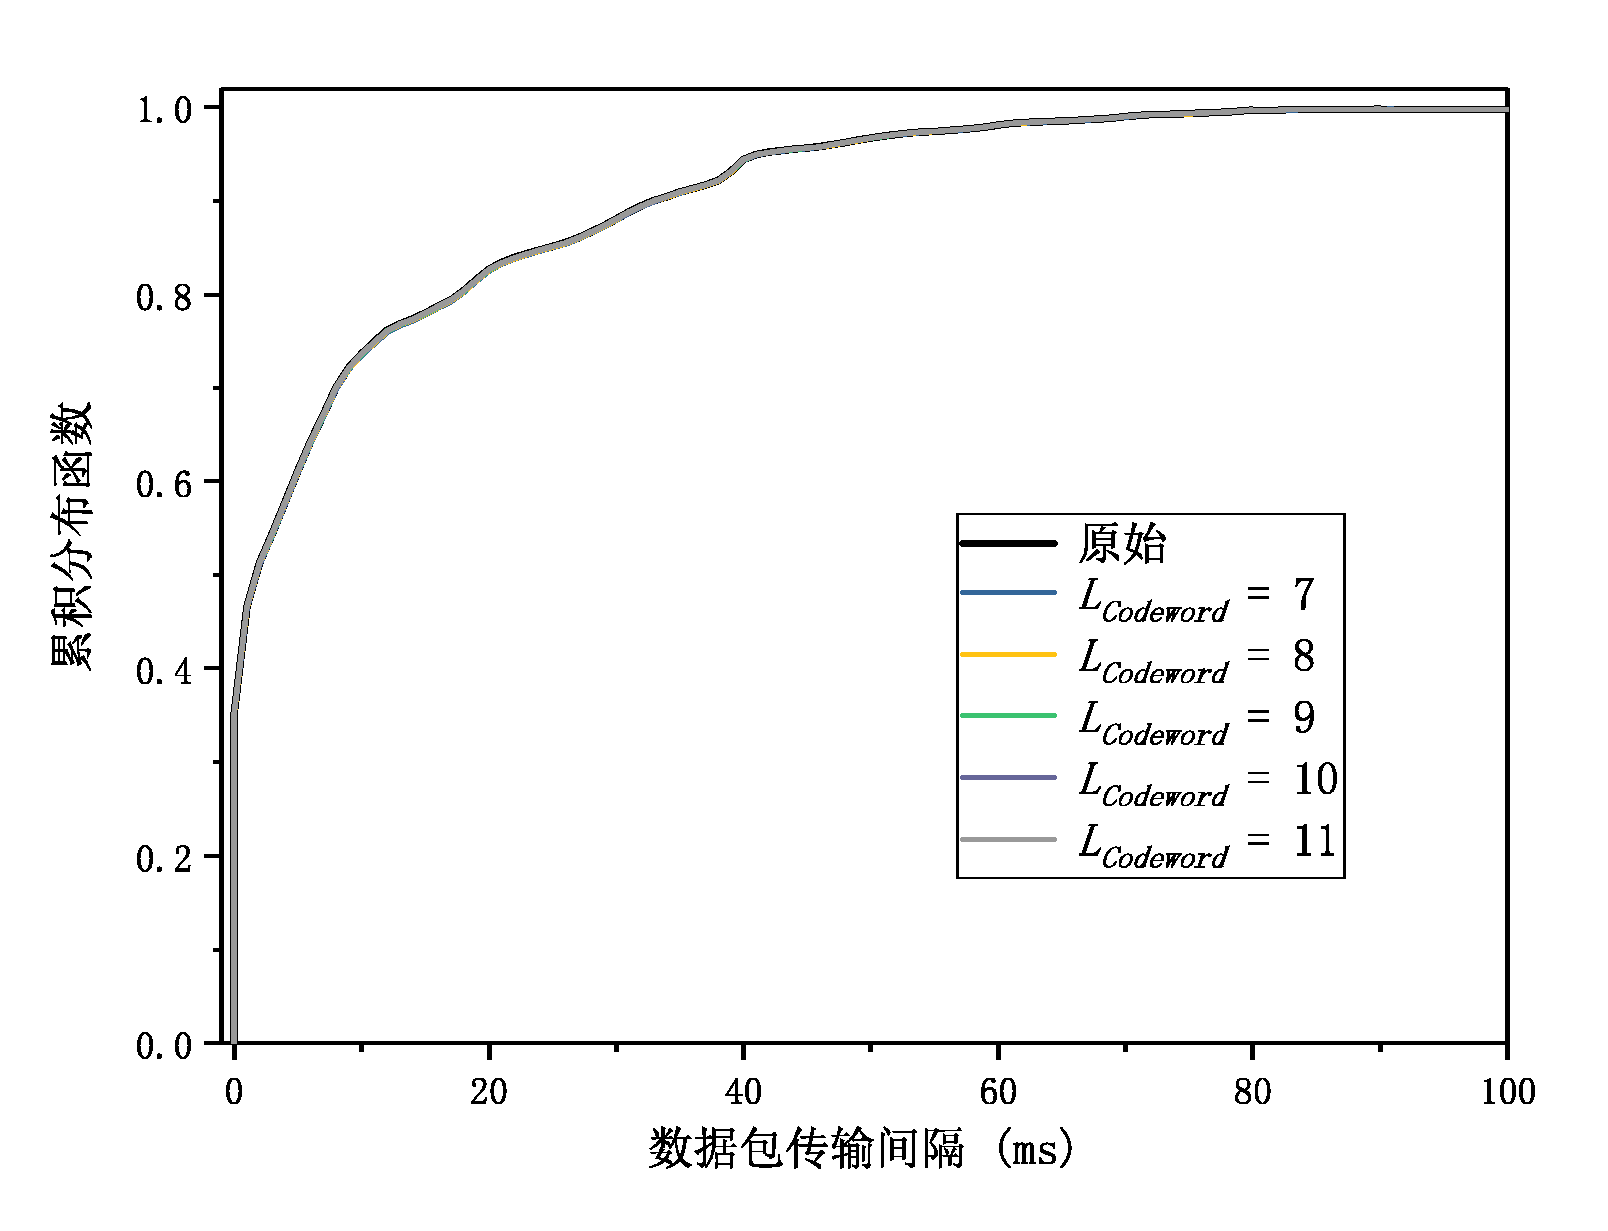
\includegraphics[width=0.48\textwidth]{chapters/chapter4/figures/ipd-cdf-excellent.pdf}
        }
        \subfigure[Good场景的CDF曲线]{
            \label{fig:4:results:ipd:cdf:good}
            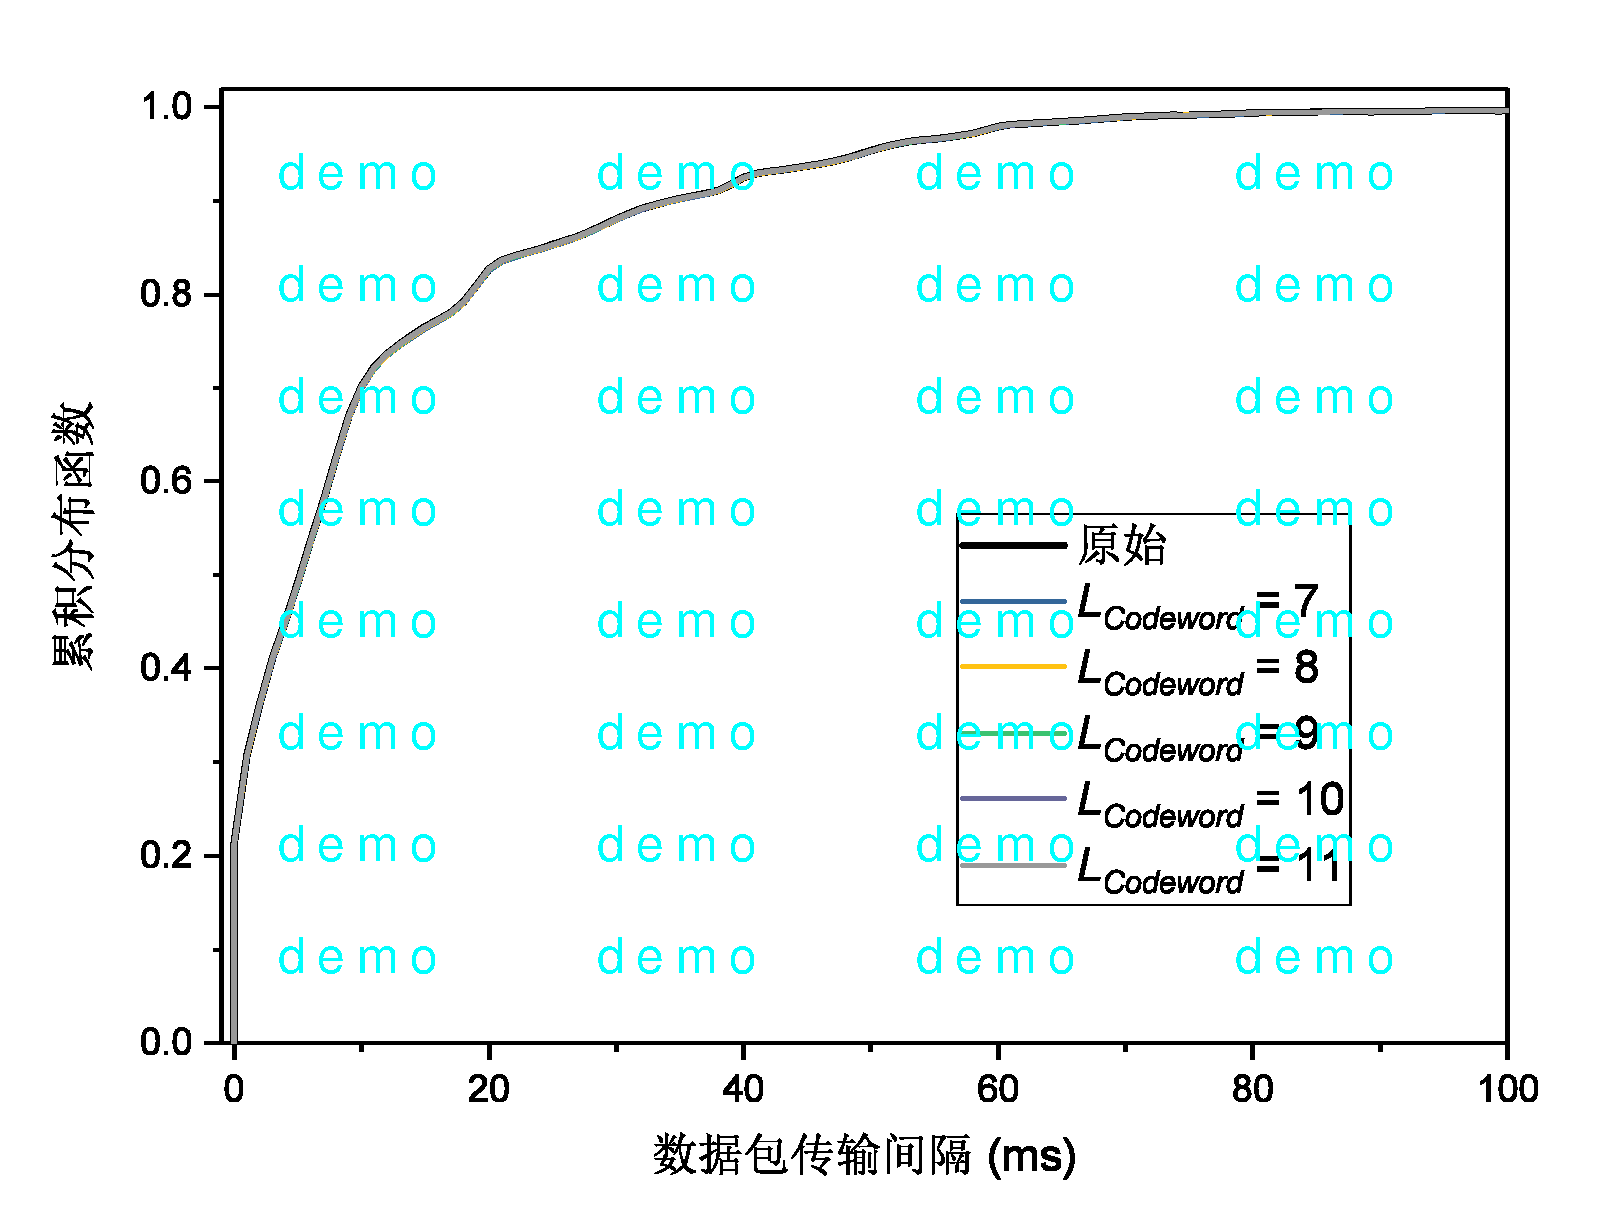
\includegraphics[width=0.48\textwidth]{chapters/chapter4/figures/ipd-cdf-good.pdf}
        }
        \caption{IPD分布的CDF曲线}
        \label{fig:4:results:ipd:cdf}
    \end{figure}
}

\insertTable{
	\begin{table}[htbp]
        \centering
        \caption{IPD检测检出率汇总表}
        \label{tab:4:results:ipd}
        \begin{threeparttable}
            \begin{tabular*}{0.85\textwidth}{@{\extracolsep{\fill}}ccc}
                \toprule
                $L_{Codeword}$ & 方法 & 检出率\\ 
                \midrule
                \multirow{5}{*}{7,\ 8,\ 9,\ 10,\ 11} 
                & K-S检验 & 0\ \% \\
                & Welch's t检验, Mann–Whitney rank检验\tnote{1} & 0\ \% \\
                & K-L散度 & 0\ \% \\
                & Wasserstein距离 & 0\ \% \\
                & 能量距离 & 0\ \% \\
                \bottomrule
            \end{tabular*}
            \begin{tablenotes}
                \footnotesize
                \item[1] Welch's t检验与Mann–Whitney rank检验通过一种即可
            \end{tablenotes}
        \end{threeparttable}
    \end{table}
}

IPD分布的CDF曲线如图\ \nref{fig:4:results:ipd:cdf}所示,不同的场景中,通过IPD的CDF曲线已经无法检测该时间隐通道。该结果与本文\ \nref{chap:analyze:result:ipd:cdf}中的测试结果一致,当$L_{Codeword}\ge 7$时,IPD分布方面已经没有可区分差异,基于IPD的检测方法无法检测出该时间隐通道。

IPD分布的量化检测结果如表\ \nref{tab:4:results:ipd},所有的测试项中,该时间隐通道均无法被检测出来。测试结果表明,该时间隐通道在IPD分布方面具备抗检测能力,满足时间隐通道的隐蔽性要求。

\subsubsection{连续丢包数检测}
\label{chap:zigzag:results:undetectability:burst}

\insertFigure{
    \begin{figure}[htbp]
        \centering
        \subfigure[Excellent场景的CDF曲线]{
            \label{fig:4:results:burst:cdf:excellent}
            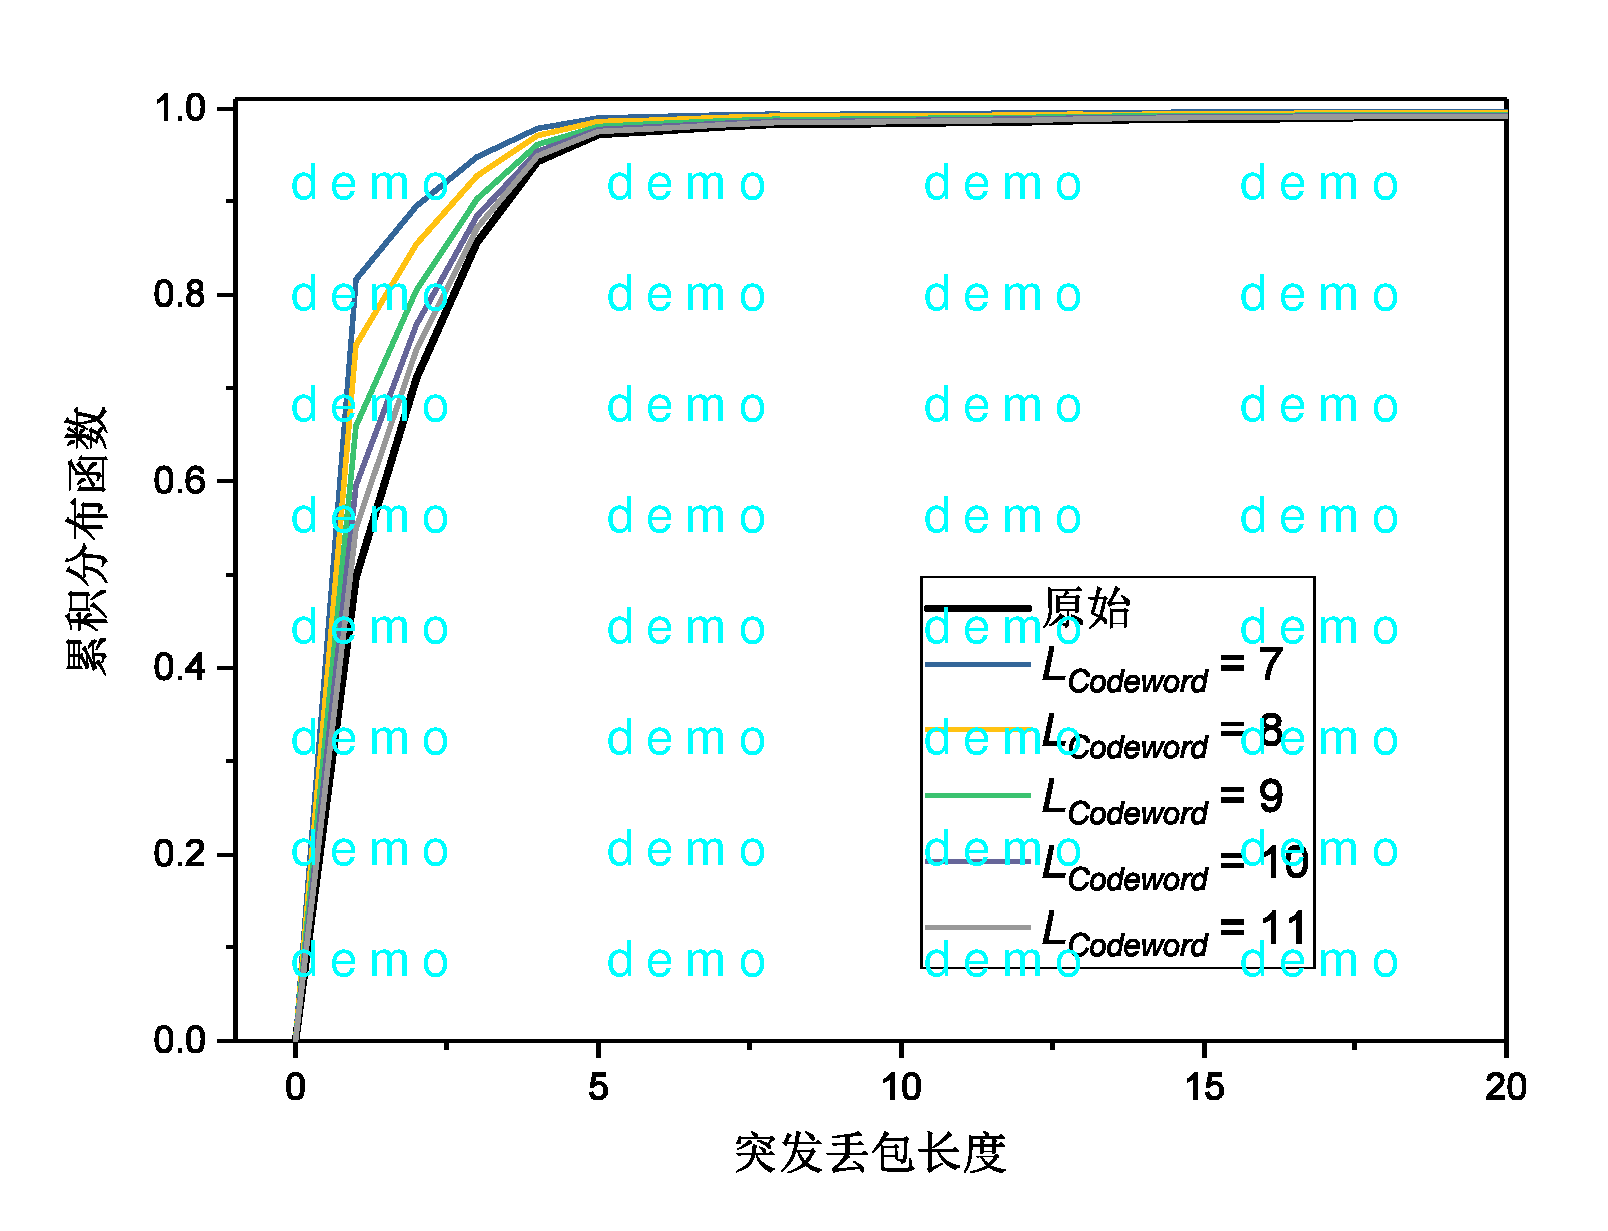
\includegraphics[width=0.48\textwidth]{chapters/chapter4/figures/burst-cdf-excellent.pdf}
        }
        \subfigure[Good场景的CDF曲线]{
            \label{fig:4:results:burst:cdf:good}
            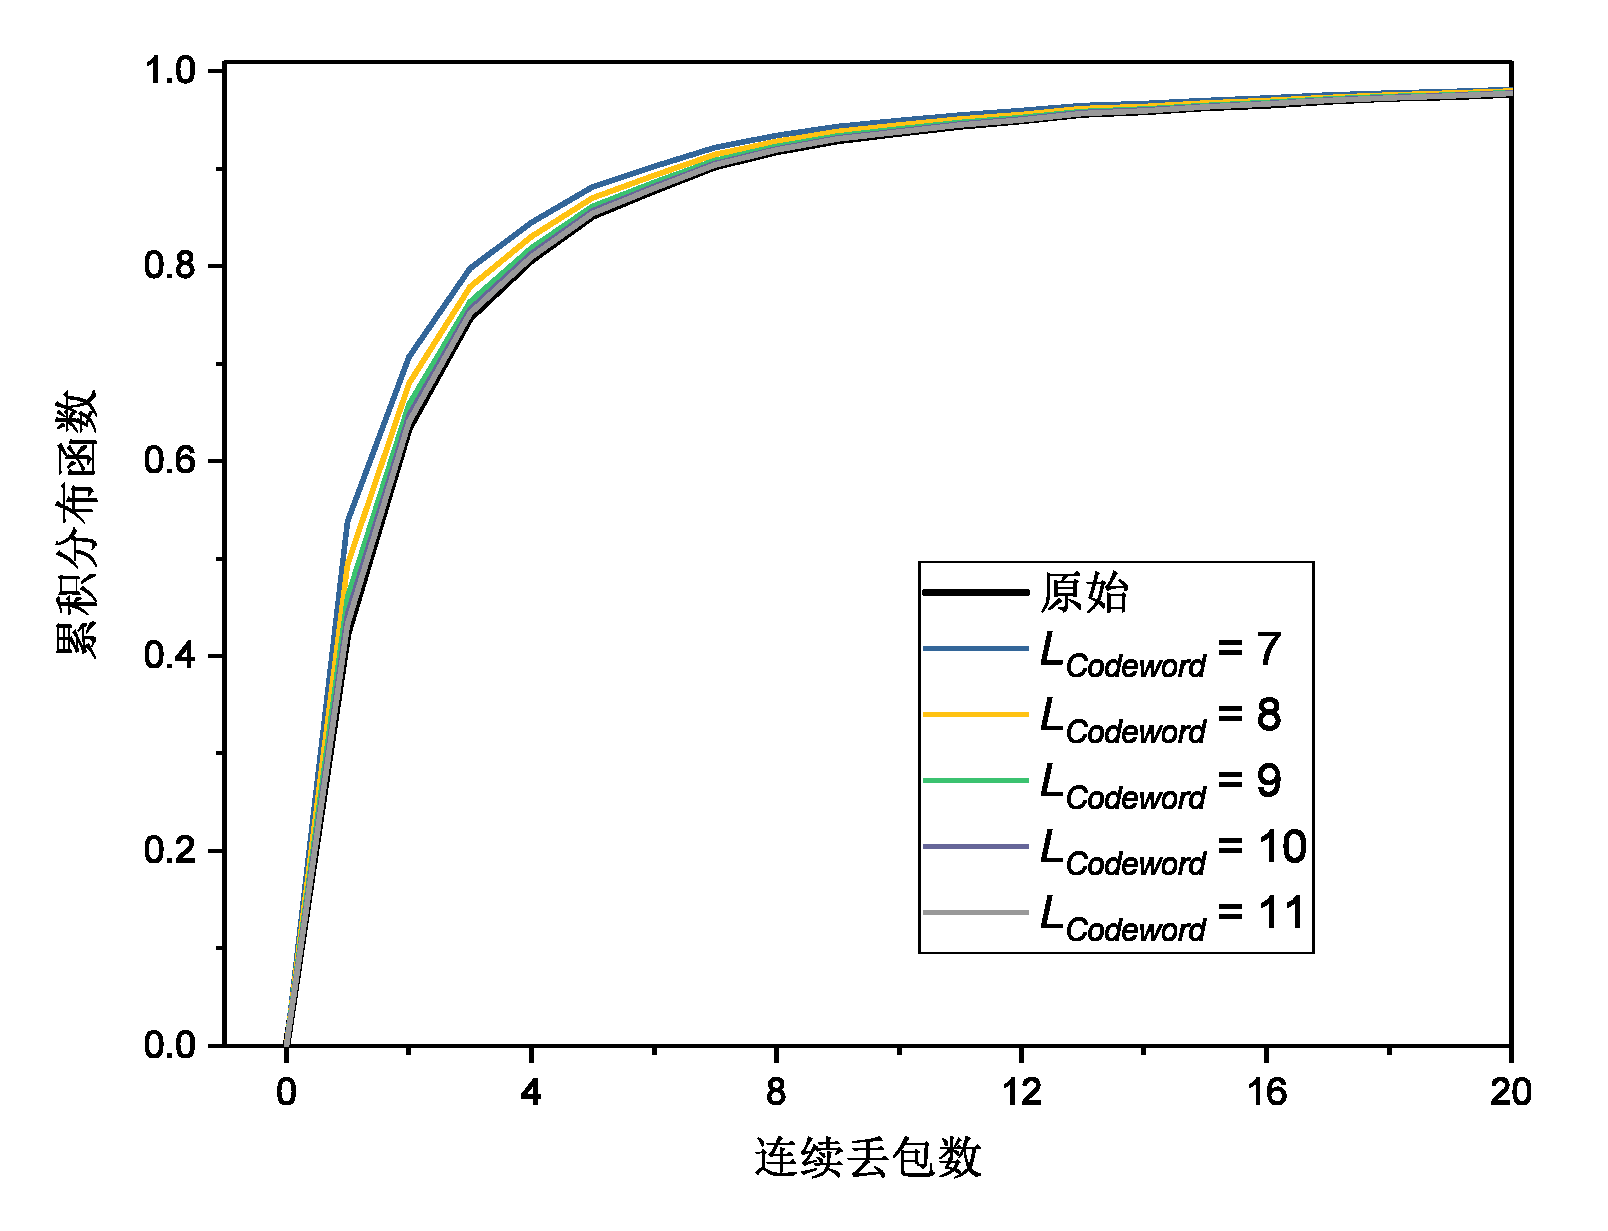
\includegraphics[width=0.48\textwidth]{chapters/chapter4/figures/burst-cdf-good.pdf}
        }
        \caption{连续丢包数的CDF曲线}
        \label{fig:4:results:burst:cdf}
    \end{figure}
}

\insertTable{
	\begin{table}[htbp]
      \centering
      \caption{连续丢包数检测检出率汇总表}
      \label{tab:4:results:burst}
          \begin{tabular*}{0.75\textwidth}{@{\extracolsep{\fill}}cccc}
            \toprule
            场景 & $L_{Codeword}$ & 方法 & 检出率 \\ 
            \midrule
            \multirow{4}{*}{Excellent} 
            & 7,\ 8 & K-L散度 & 100\ \% \\
            & 9,\ 10,\ 11 & K-L散度 & 0\ \% \\
            & 7,\ 8,\ 9,\ 10,\ 11 & Wasserstein距离 & 0\ \% \\
            & 7,\ 8,\ 9,\ 10,\ 11 & 能量距离 & 0\ \% \\
            \\
            \multirow{3}{*}{Good}
            & 7,\ 8,\ 9,\ 10,\ 11 & K-L散度 & 0\ \% \\
            & 7,\ 8,\ 9,\ 10,\ 11 & Wasserstein距离 & 0\ \% \\
            & 7,\ 8,\ 9,\ 10,\ 11 & 能量距离 & 0\ \% \\
            \bottomrule
          \end{tabular*}
    \end{table}
}

连续丢包数的CDF曲线,如图\ \nref{fig:4:results:burst:cdf}。两种场景中,时间隐通道的曲线均出现了一定偏离,并且Excellent场景中的差异明显。总体来说,随着$L_{Codeword}$增大,时间隐通道的分布与原始分布更加接近。参照表\ \nref{tab:4:parameters},主动丢包率与参数$L_{Codeword}$呈负相关,减少丢包则对分布的影响减弱。

连续丢包数检测的量化评估结果,如表\ \nref{tab:4:results:burst}。Excellent场景中,当$L_{Codeword}\ge 9$时,已经无法检测出时间隐通道;而Good场景中,设定的参数下已经无法检测出时间隐通道。因此,Excellent场景下$L_{Codeword}$至少为9,而Good场景下$L_{Codeword}\ge 7$即可满足要求。

\subsubsection{区间丢包数检测}
\label{chap:zigzag:results:undetectability:win}

\insertFigure{
    \begin{figure}[htbp]
        \centering
        \subfigure[区间长度为100时Excellent场景的CDF曲线]{
            \label{fig:4:results:win100:cdf:excellent}
            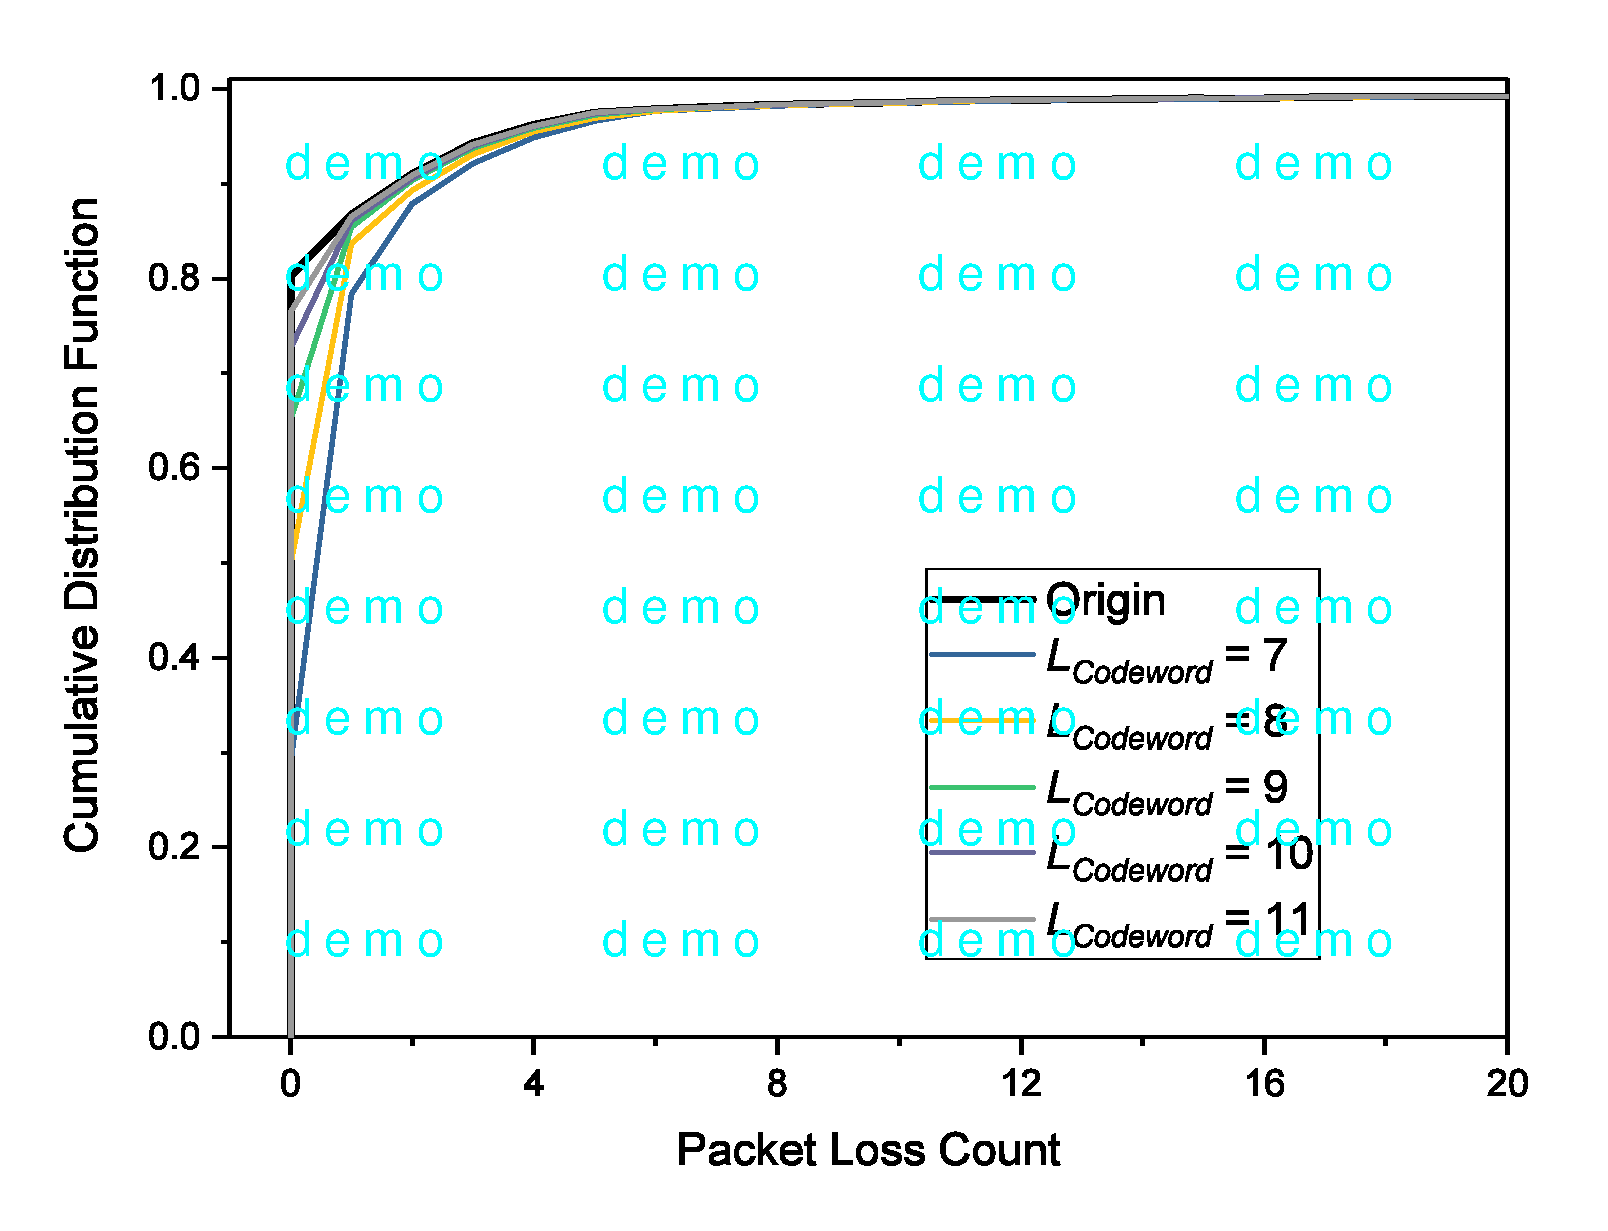
\includegraphics[width=0.48\textwidth]{chapters/chapter4/figures/win100-cdf-excellent.pdf}
        }
        \subfigure[区间长度为100时Good场景的CDF曲线]{
            \label{fig:4:results:win100:cdf:good}
            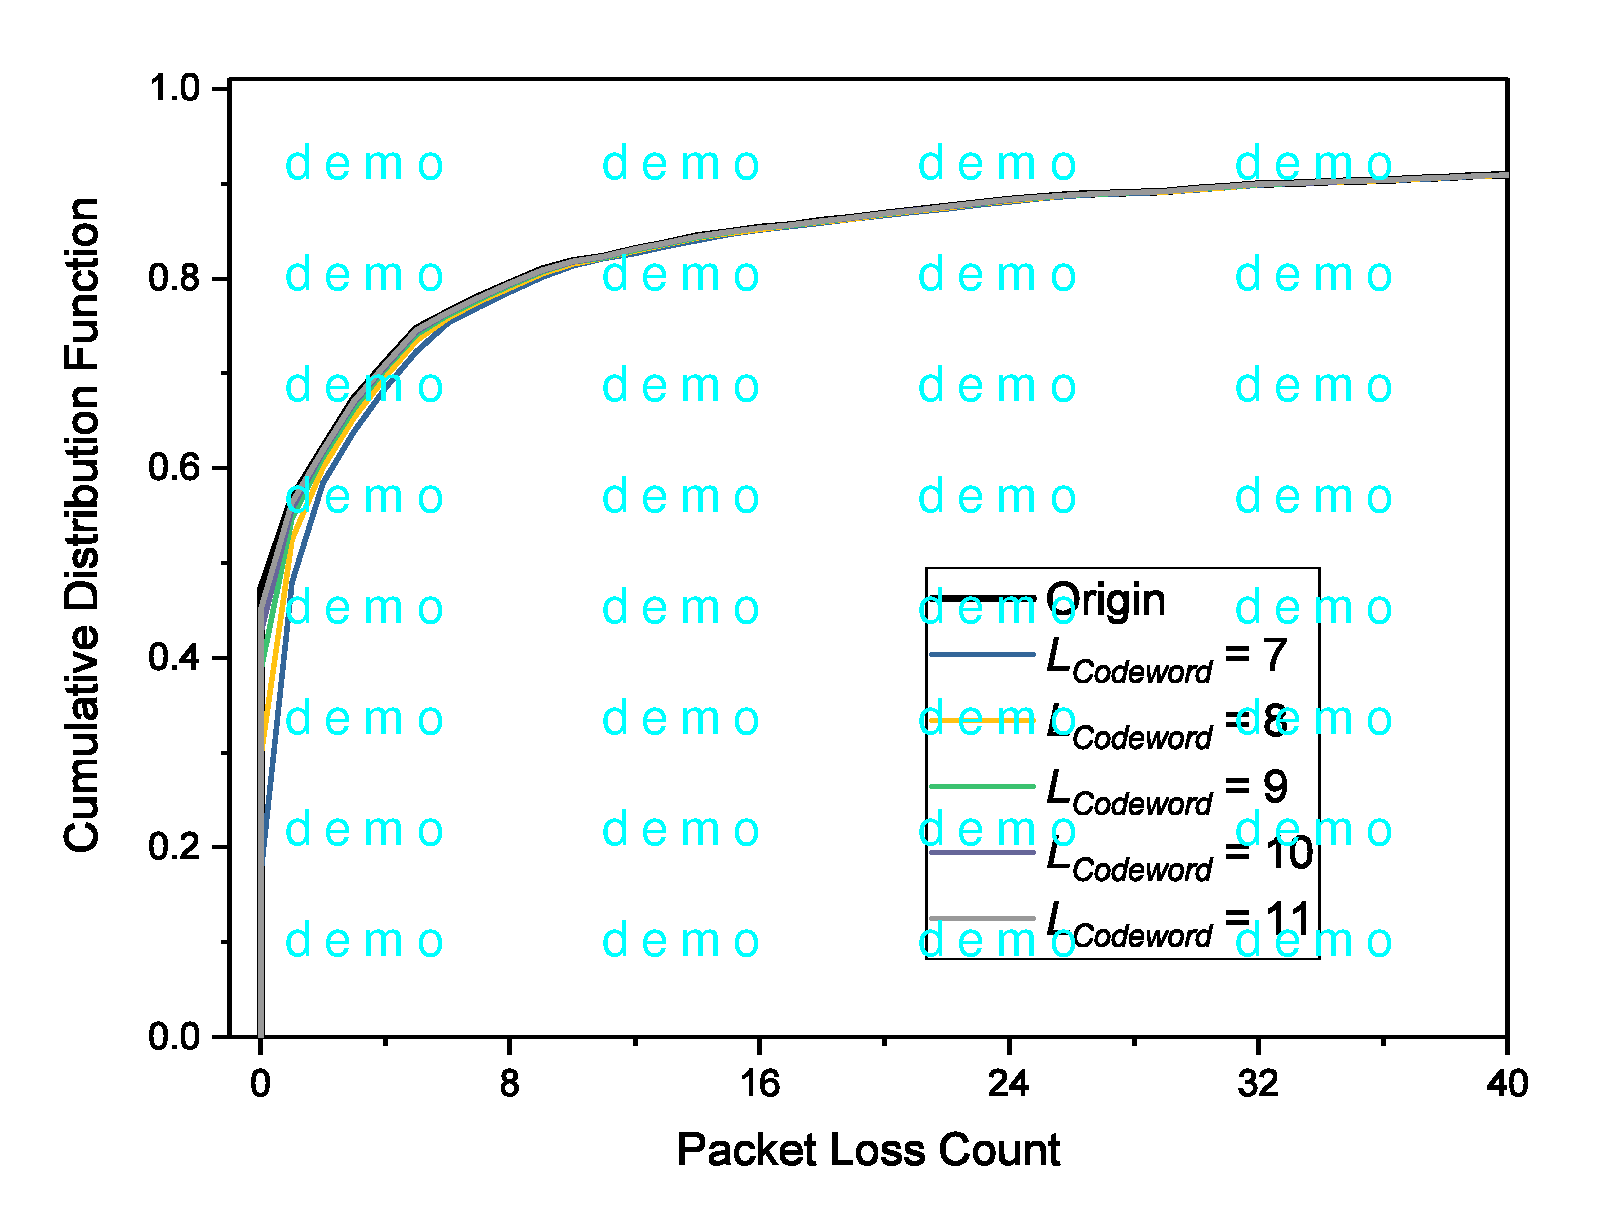
\includegraphics[width=0.48\textwidth]{chapters/chapter4/figures/win100-cdf-good.pdf}
        }
        \subfigure[区间长度为200时Excellent场景的CDF曲线]{
            \label{fig:4:results:win200:cdf:excellent}
            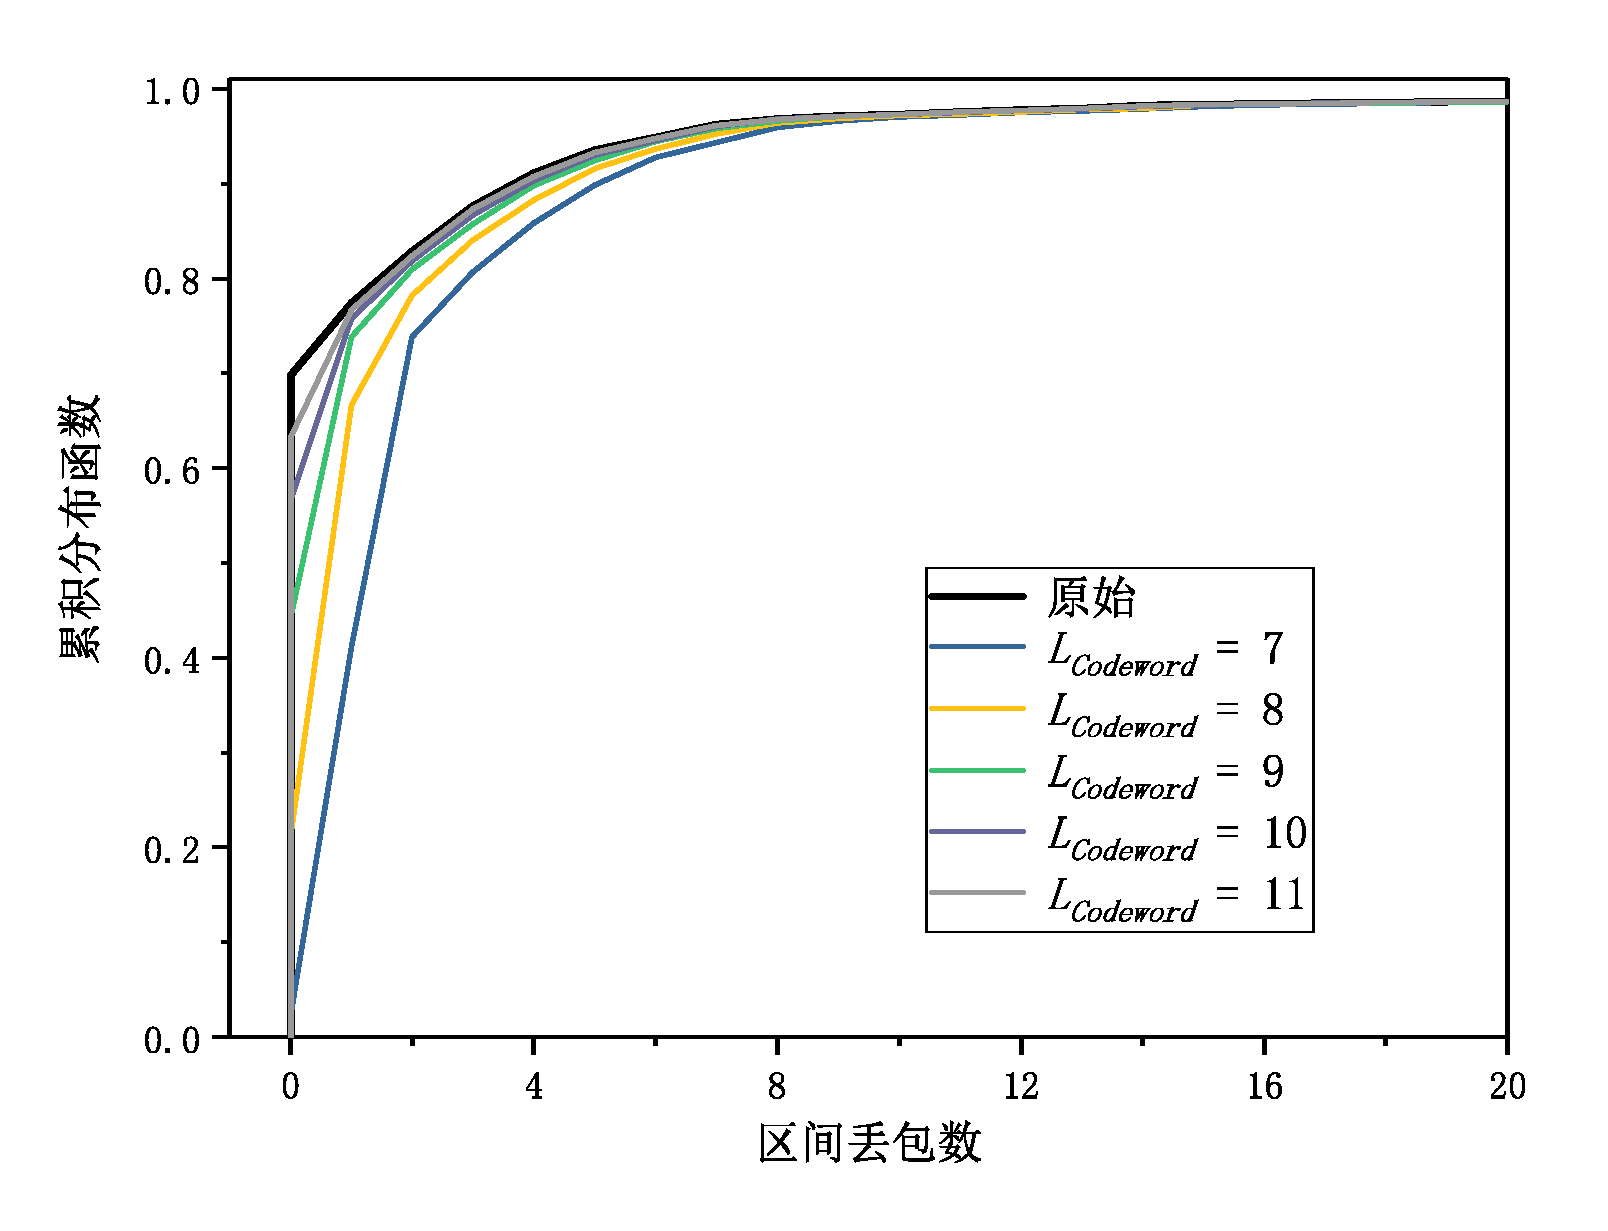
\includegraphics[width=0.48\textwidth]{chapters/chapter4/figures/win200-cdf-excellent.pdf}
        }
        \subfigure[区间长度为200时Good场景的CDF曲线]{
            \label{fig:4:results:win200:cdf:good}
            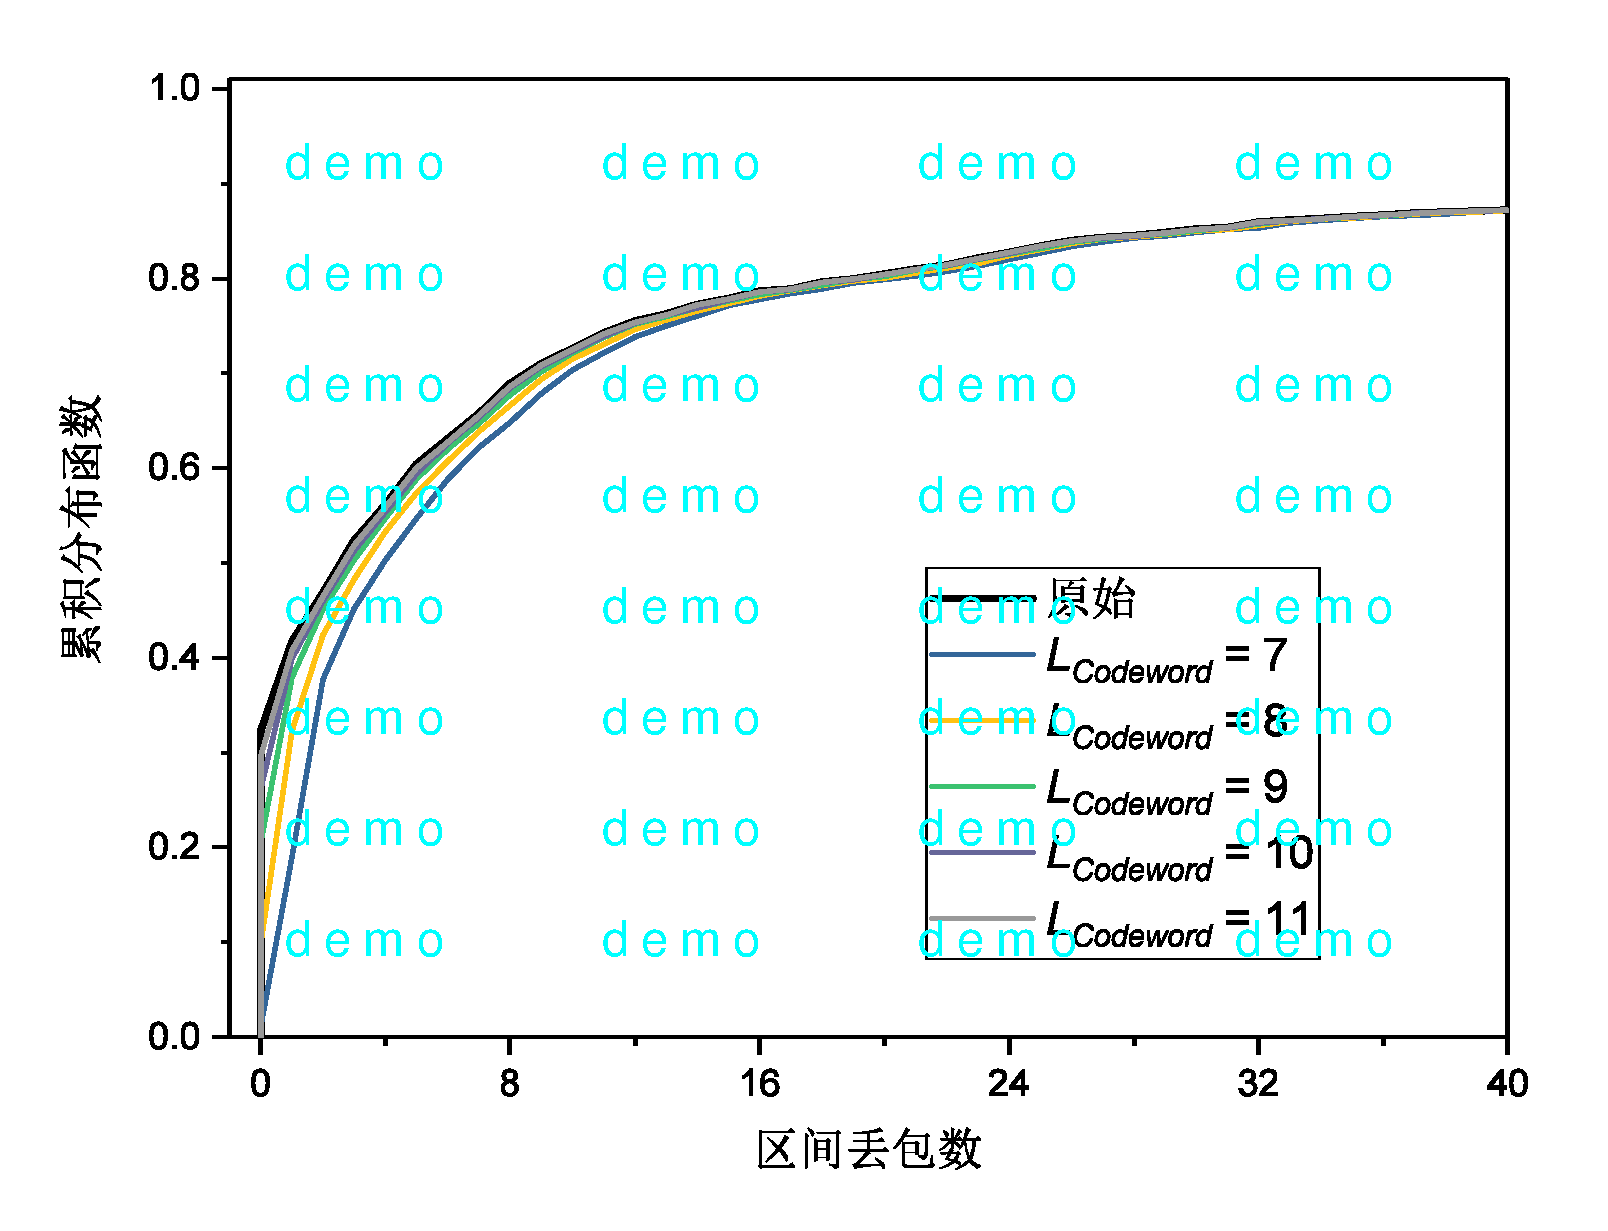
\includegraphics[width=0.48\textwidth]{chapters/chapter4/figures/win200-cdf-good.pdf}
        }
        \caption{区间丢包数的CDF曲线}
        \label{fig:4:results:win:cdf}
    \end{figure}
}

\insertTable{
	\begin{table}[htbp]
      \centering
      \caption{区间丢包数检测检出率汇总表}
      \label{tab:4:results:win}
          \begin{tabular*}{0.75\textwidth}{@{\extracolsep{\fill}}cccc}
            \toprule
            场景 & $L_{Codeword}$ & 方法 & 检出率 \\ 
            \midrule
            \multirow{4}{*}{Excellent} 
            & 7 & Wasserstein距离 & 100\ \% \\
            & 8,\ 9,\ 10,\ 11 & Wasserstein距离 & 0\ \% \\
            & 7 & 能量距离 & 100\ \% \\
            & 8,\ 9,\ 10,\ 11 & 能量距离 & 0\ \% \\
            \\
            \multirow{6}{*}{Good}
            & 7 & Wasserstein距离 & 100\ \% \\
            & 8 & Wasserstein距离 & 30\ \% \\
            & 9,\ 10,\ 11 & Wasserstein距离 & 0\ \% \\
            & 7 & 能量距离 & 100\ \% \\
            & 8 & 能量距离 & 30\ \% \\
            & 9,\ 10,\ 11 & 能量距离 & 0\ \% \\
            \bottomrule
          \end{tabular*}
    \end{table}
}

区间丢包数检测中,区间长度与本文\ \nref{chap:analyze:result:window}保持一致,分别为100及200。区间丢包数的CDF曲线如图\ \nref{fig:4:results:win:cdf},本时间隐通道的CDF曲线出现部分偏离,与本文\ \nref{chap:analyze:result:window}的检测结果基本一致。

区间丢包数检测的量化结果,如表\ \nref{tab:4:results:win},Wasserstein距离及能量距离具备良好检测能力。Excellent场景下,当$L_{Codeword}\ge 8$时即可通过检测;而Good场景下,当$L_{Codeword}\ge 9$时才通过所有检测。

\subsubsection{抗检测能力测试汇总}
\label{chap:zigzag:results:undetectability:all}

\insertTable{
	\begin{table}[htbp]
      \centering
      \caption{基于Zigzag映射矩阵的时间隐通道检出率汇总表}
      \label{tab:4:results:sum}
          \begin{tabular*}{0.8\textwidth}{@{\extracolsep{\fill}}cccccc}
            \toprule
            \multirow{2.5}{*}{场景} 
            & \multicolumn{5}{c}{$L_{Codeword}$} \\
            \cmidrule(l){2-6}
            & 7 & 8 & 9 & 10 & 11 \\
            \midrule
            Excellent & 100\ \% & 100\ \% & 0\ \% & 0\ \% & 0\ \% \\
            Good & 100\ \% & 30\ \% & 0\ \% & 0\ \% & 0\ \% \\
            \bottomrule
          \end{tabular*}
    \end{table}
}

基于Zigzag映射矩阵的时间隐通道,其抗检测能力测试的最终结果如表\ \nref{tab:4:results:sum}。当$L_{Codeword}\ge 9$时,即可通过所有检测;当$L_{Codeword} = 8$时,Good场景下有一定几率通过检测。通过对比实验结果,Excellent场景对主动丢包的容忍度有限,传输参数需要保守设定。

通过分析抗检测能力测试结果,本方法通过调整参数$L_{Codeword}$,在各种通话场景下均可通过测试。测试结果与表\ \nref{tab:3:result-sum:all}基本一致,同时验证了该构建方法及时间隐通道检测方法。

\subsection{鲁棒性测试}
\label{chap:zigzag:results:robustness}

\insertFigure{
	\begin{figure}[htbp]
        \centering
        \subfigure[Excellent场景及Good场景]{
            \label{fig:4:results:ber:scenario}
            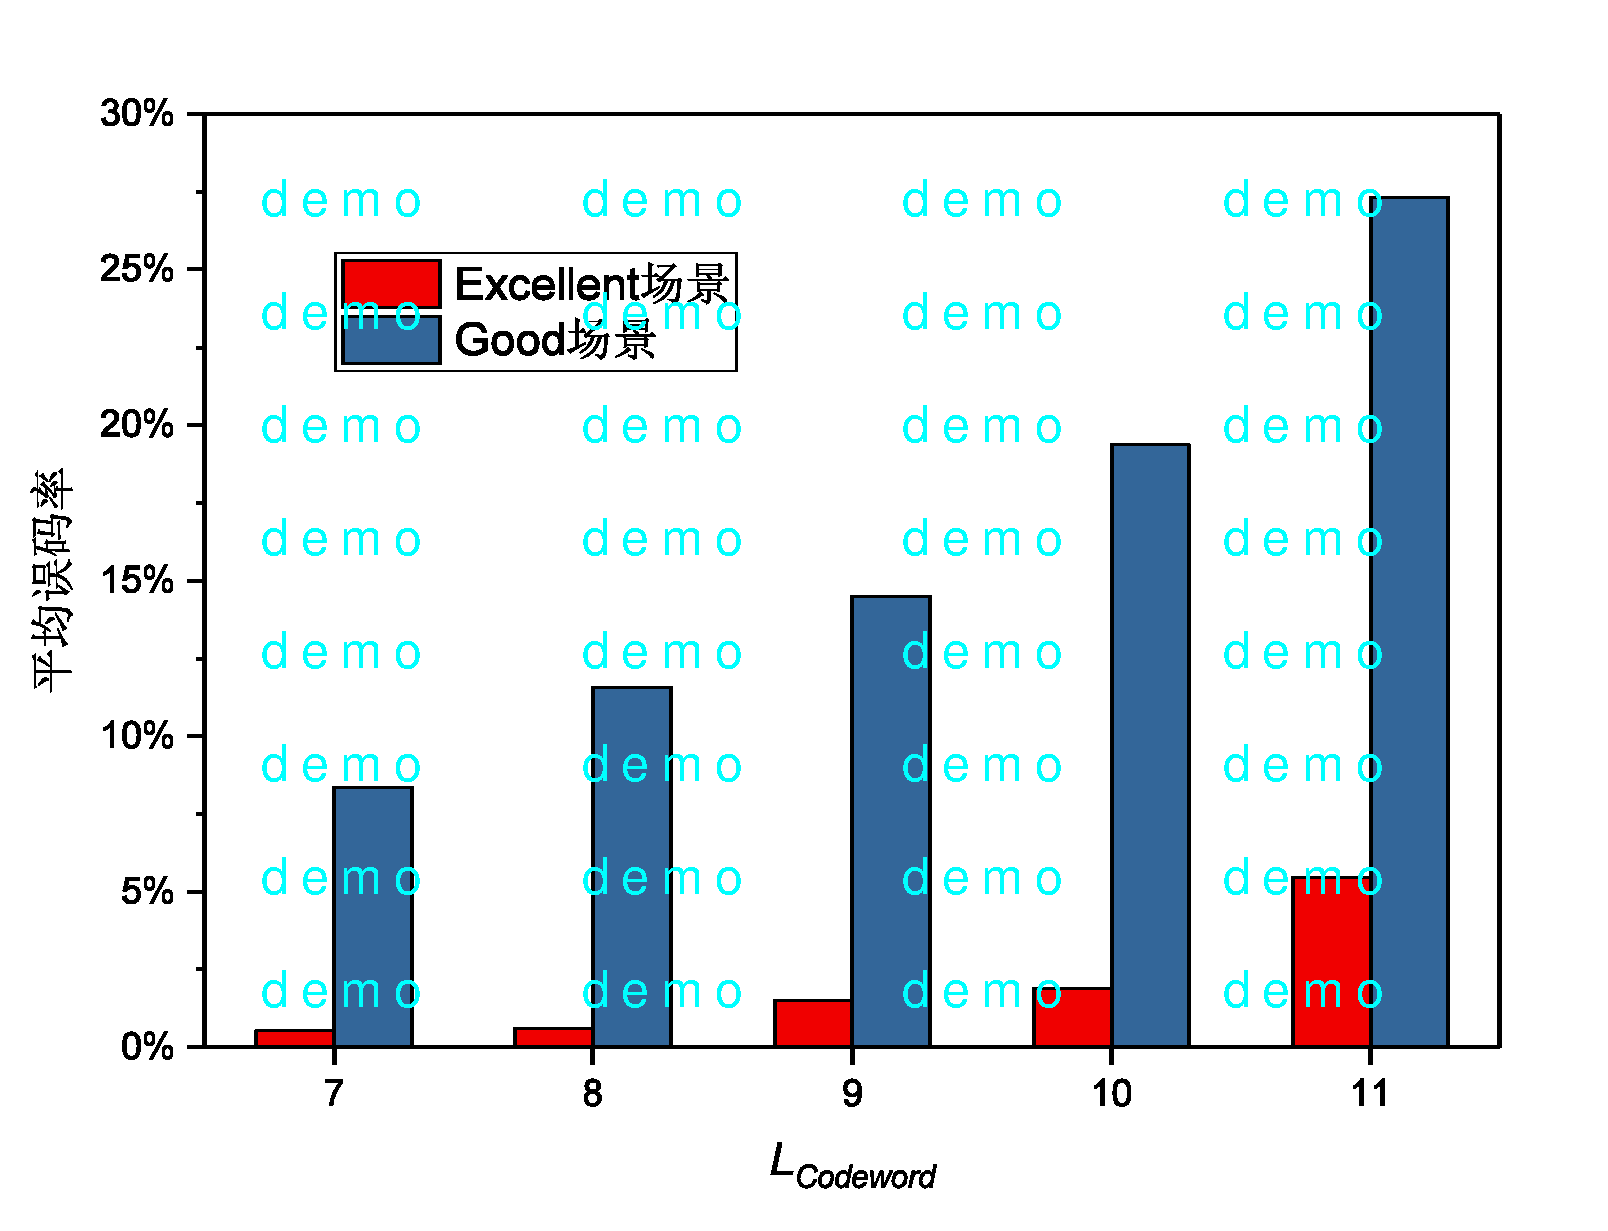
\includegraphics[width=0.48\textwidth]{chapters/chapter4/figures/ber-scenarios.pdf}
        }
        \subfigure[随机噪声场景]{
            \label{fig:4:results:ber:random}
            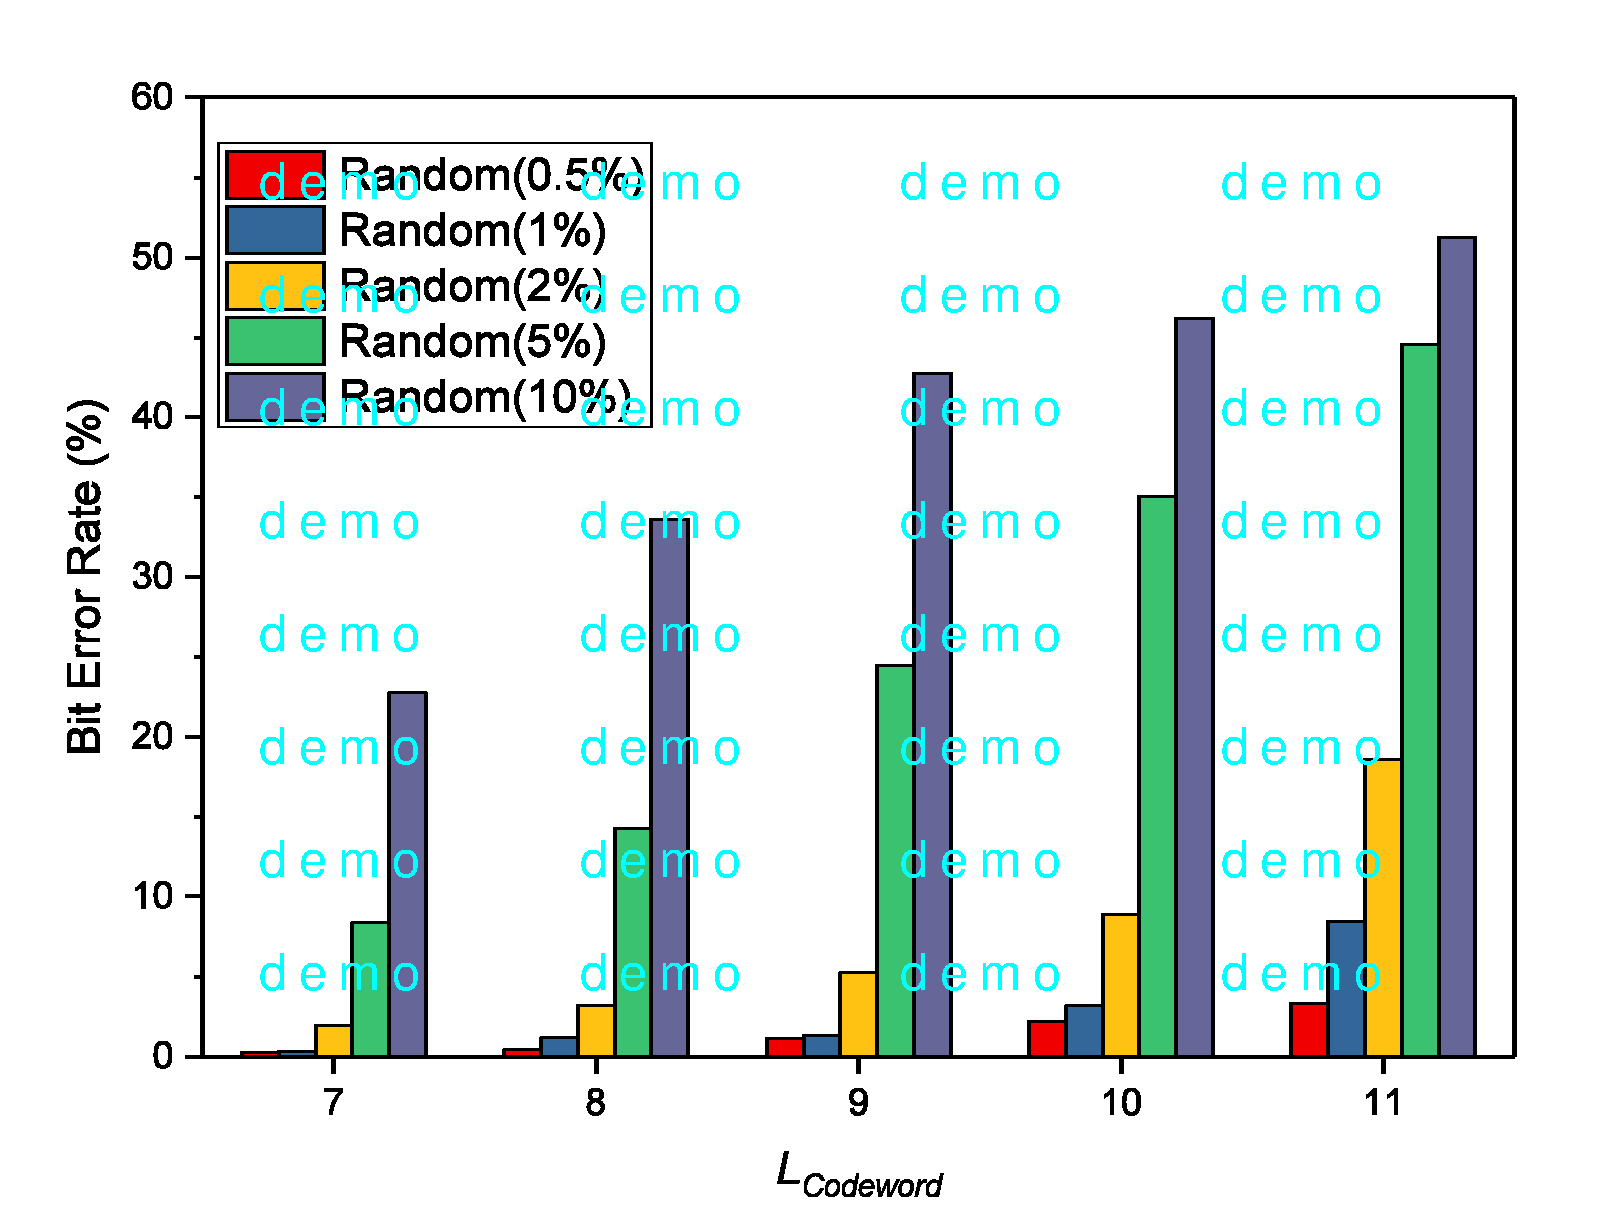
\includegraphics[width=0.48\textwidth]{chapters/chapter4/figures/ber-random.pdf}
        }
        \caption{时间隐通道的误码率水平}
        \label{fig:4:results:ber}
    \end{figure}
}

根据公式(\nref{equ:2:ber}),误码率BER(Bit Error Rate)是评估鲁棒性的基本方式。各场景下的误码率水平如图\ \nref{fig:4:results:ber},其中图\ \nref{fig:4:results:ber:scenario}为Excellent场景及Good场景的测试结果,图\ \nref{fig:4:results:ber:random}为随机噪声场景的测试结果。

根据测试结果,随着$L_{Codeword}$的增长,误码率水平增加。由于$L_{Codeword}$ bits的数据需要$2^{L_{Codeword}}$个数据包完成调制,因此增大$L_{Codeword}$导致累积丢包数增加,码字鉴别准确率降低,时间隐通道的鲁棒性减弱,误码率升高。

网络噪声,尤其是随机丢包影响该时间隐通道,导致误码率与随机丢包率呈正相关。对比图\ \nref{fig:4:results:ber:random}中随机噪声下的误码率,Excellent场景与{$1\ \%$}随机噪声的结果相近,Good场景与{$10\ \%$}随机噪声的结果相近,与数据集的平均丢包率基本一致(表\ \nref{tab:3:capture-results})。测试结果表明,随机丢包是对该时间隐通道的主要干扰。

在满足抗检测能力要求,即$L_{Codeword}\ge 9$的基础上,该时间隐通道在Excellent场景下可以保证{$2\ \%$}左右的误码率;Good场景中误码率水平上升至{$15\ \%$}左右,对传输可靠性存在考验。因此,该时间隐通道适用于网络状况较好的场景,高噪声场景中无法保证消息无误码。

\subsection{传输性能测试}
\label{chap:zigzag:results:throughput}

\insertTable{
	\begin{table}[htbp]
      \centering
      \caption{基于Zigzag映射矩阵时间隐通道的传输性能}
      \label{tab:4:results:throughput}
          \begin{tabular*}{0.8\textwidth}{@{\extracolsep{\fill}}cccccc}
            \toprule
            \multirow{2.5}{*}{指标} 
            & \multicolumn{5}{c}{$L_{Codeword}$} \\
            \cmidrule(l){2-6}
            & 7 & 8 & 9 & 10 & 11 \\
            \midrule
            传输速率\ (bps) & 2.73 & 1.56 & 0.88 & 0.49 & 0.27 \\
            信道容量\ (bpp) & 0.027 & 0.016 & 0.009 & 0.005 & 0.003 \\
            \bottomrule
          \end{tabular*}
    \end{table}
}

根据公式(\nref{equ:4:throughput}),该时间隐通道的传输性能只与参数$L_{Codeword}$有关。不同参数下的传输性能如表\ \nref{tab:4:results:throughput},传输速率与$L_{Codeword}$呈负相关。在满足隐蔽性前提下,当$L_{Codeword}=9$时,达到最高性能{0.88\ bps},增大$L_{Codeword}$导致性能衰减。

由传输性能考虑,降低$L_{Codeword}$能够有效提升传输速率,但代价是抗检测能力的衰退,违背了时间隐通道的原则。尤其是对基于主动丢包的时间隐通道来说,主动丢弃的数据包越多,用户通话质量受到的影响越大,对隐蔽性的损害越大。

\subsection{构建代价测试}
\label{chap:zigzag:results:cost}

\insertFigure{
	\begin{figure}[htbp]
        \centering
        \subfigure[Excellent场景的视频质量]{
            \label{fig:4:results:vq-excellent}
            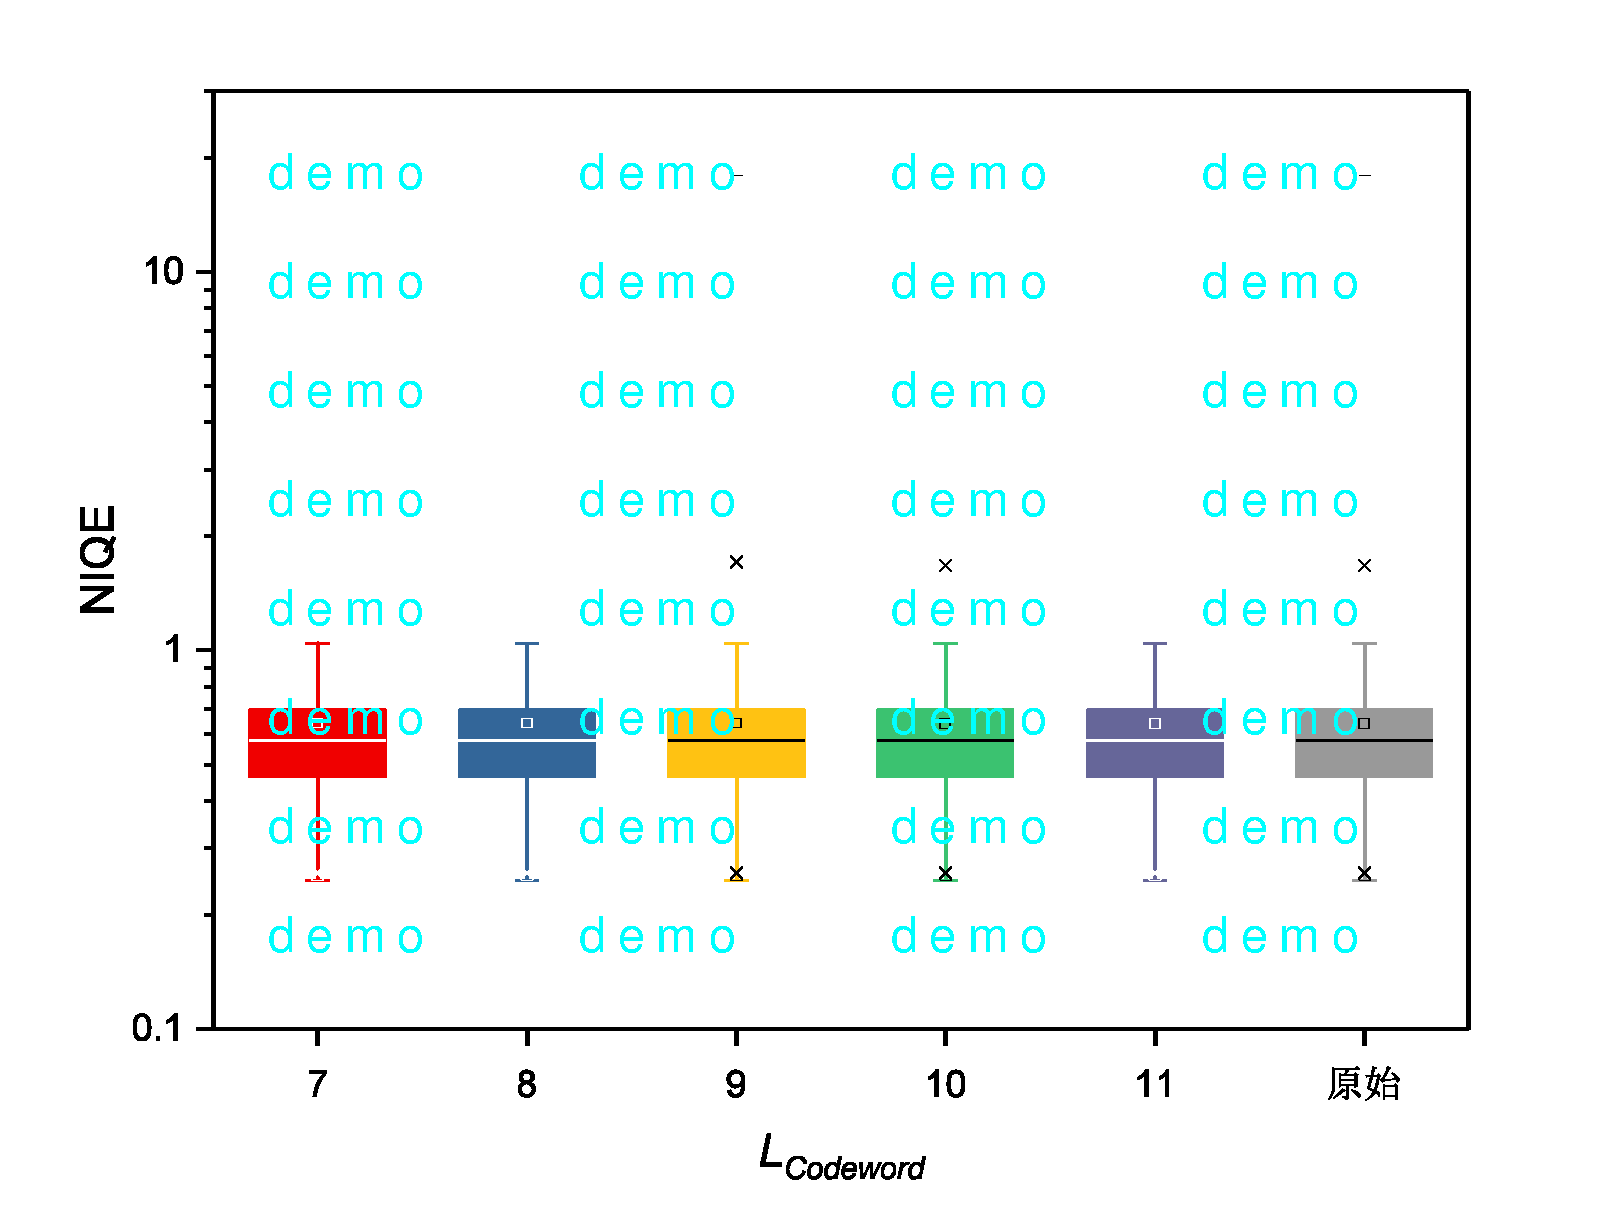
\includegraphics[width=0.48\textwidth]{chapters/chapter4/figures/vq-excellent.pdf}
        }
        \subfigure[Good场景的视频质量]{
            \label{fig:4:results:vq-good}
            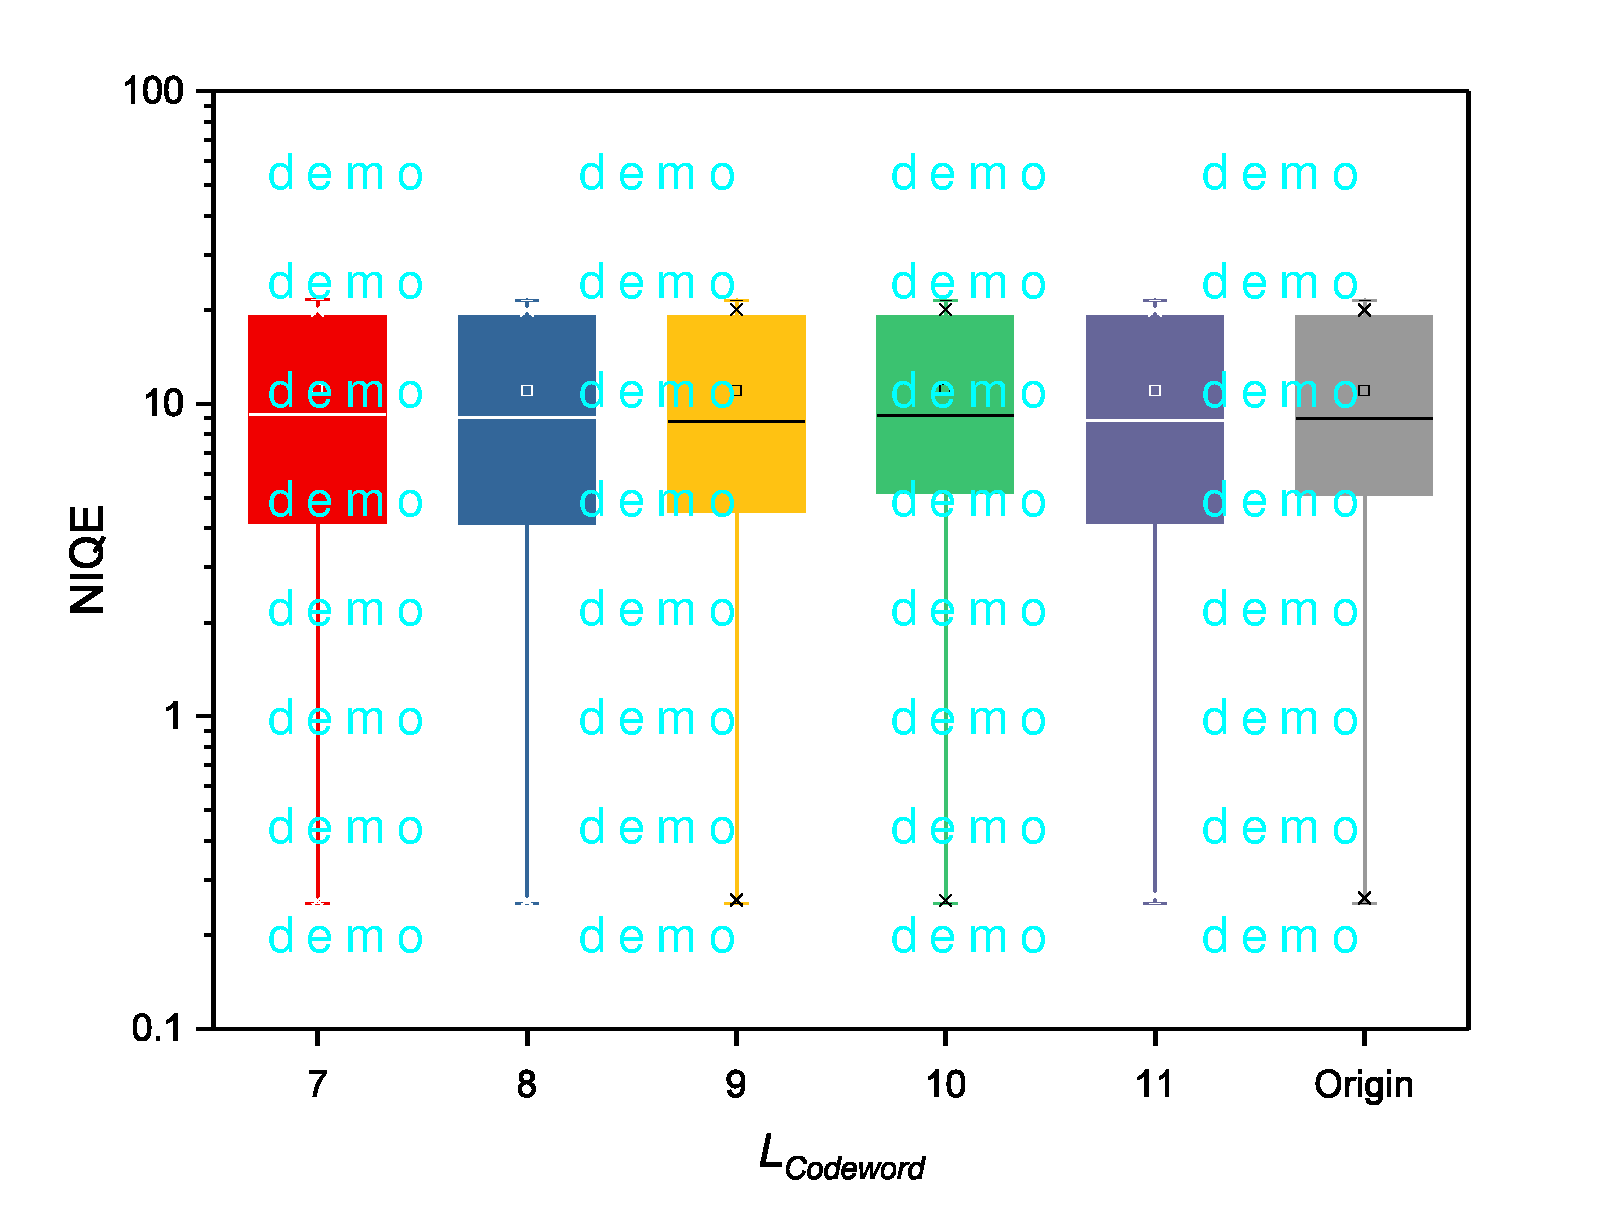
\includegraphics[width=0.48\textwidth]{chapters/chapter4/figures/vq-good.pdf}
        }
        \caption{时间隐通道的NIQE视频质量评估结果}
        \label{fig:4:results:vq}
    \end{figure}
}

基于Zigzag映射矩阵的时间隐通道,建立在VoLTE视频信道中,因此接收方视频质量是评估构建代价的重要方面。根据表\ \nref{tab:4:parameters},当$L_{Codeword}\ge 9$时,构建时间隐通道导致的丢包率低于$0.2\ \%$,远小于网络噪声产生的丢包比例,因此视频质量的变化有限。

为评估视频质量,采用NIQE(Natural Image Quality Evaluator)无参照客观评价指标\nupcite{7094273},对视频的所有帧进行评估,并判断视频整体的质量是否发生变化\nupcite{7122356}。NIQE反映了图像的失真程度,计算结果与图像质量呈反比\nupcite{CoDLaCDAfMI,10.1145/3210424.3210434,6353522}。视频质量评估结果如图\ \nref{fig:4:results:vq},Good场景下平均NIQE值高于Excellent场景,而时间隐通道导致的变化幅度较小。

两种场景中,通过对比NIQE图像质量的范围和均值,证明了时间隐通道没有产生显著视频质量损失。Excellent场景中,得益于较好的传输质量,时间隐通道产生的影响有限。Good场景中,原始的视频质量已经处于较差水平,虽然时间隐通道导致NIQE值产生了部分改变,但总体没有出现差异。通过对比,该时间隐通道不会导致视频质量发生显著改变,满足时间隐通道低代价的要求。

\subsection{结论}
\label{chap:zigzag:results:conclusion}

\insertFigure{
	\begin{figure}[htbp]
        \centering
        \subfigure[Excellent场景的综合评估]{
            \label{fig:4:results:sum:excellent}
            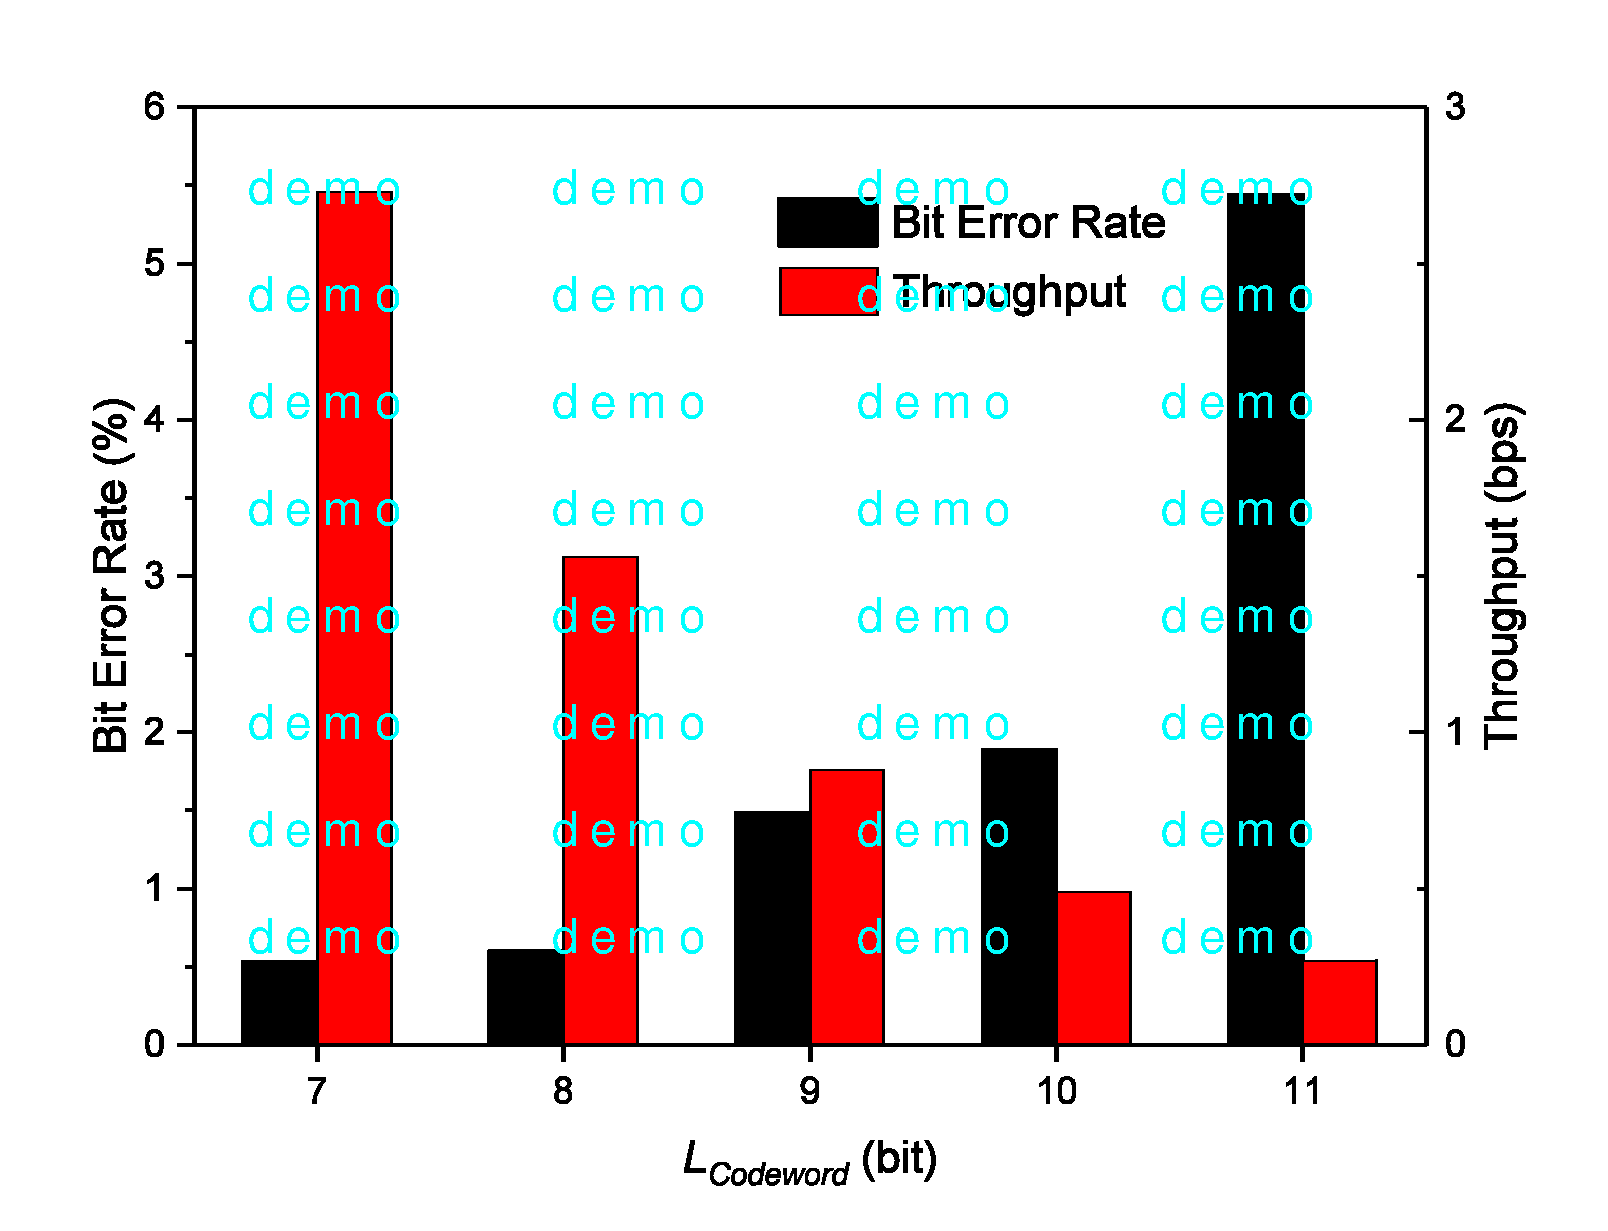
\includegraphics[width=0.48\textwidth]{chapters/chapter4/figures/sum-excellent.pdf}
        }
        \subfigure[Good场景的综合评估]{
            \label{fig:4:results:sum:good}
            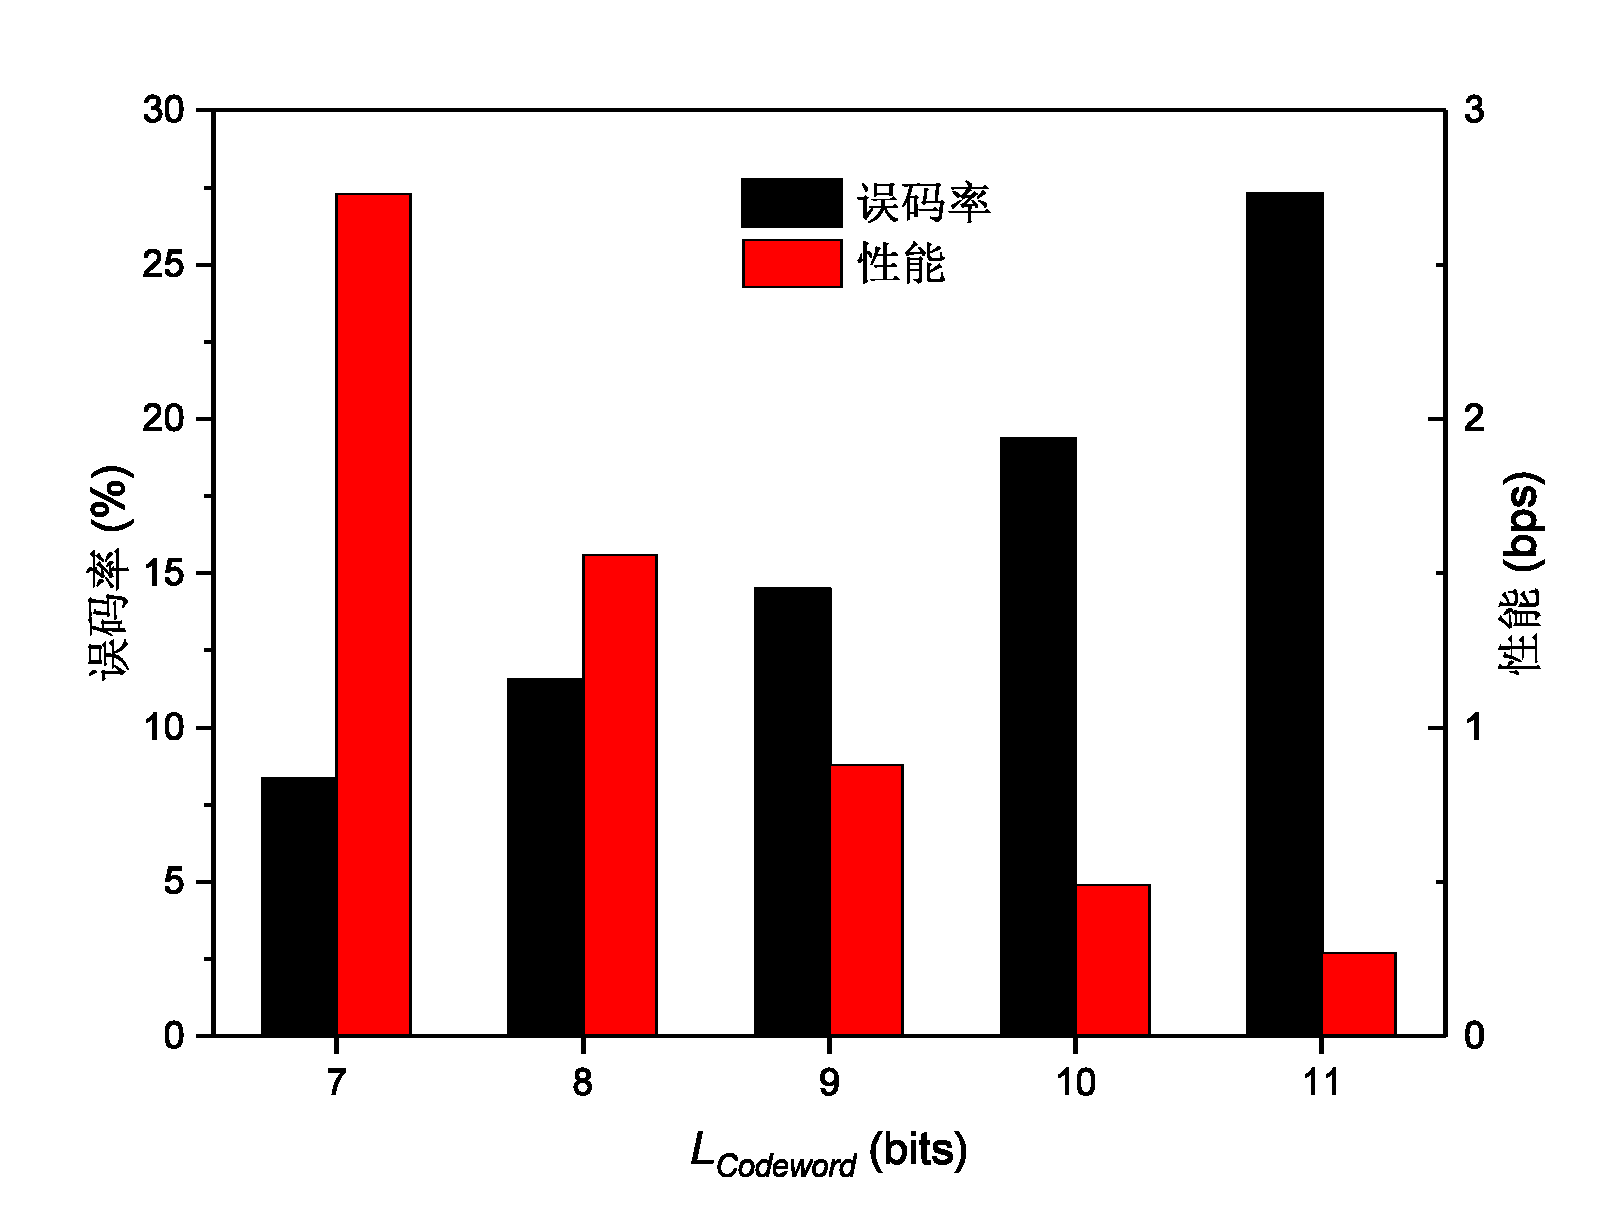
\includegraphics[width=0.48\textwidth]{chapters/chapter4/figures/sum-good.pdf}
        }
        \caption{基于Zigzag映射矩阵的时间隐通道综合评估}
        \label{fig:4:results:sum}
    \end{figure}
}

如图\ \nref{fig:4:results:sum},该时间隐通道的鲁棒性和传输性能均与$L_{Codeword}$呈负相关。结合本文\ \nref{chap:zigzag:results:undetectability}抗检测能力评估结果,该时间隐通道的最优$L_{Codeword}$为9,在该参数下能够通过所有的抗检测能力测试,并且具有{0.88\ bps}的传输性能及{1.5\ \%}的误码率。

\insertTable{
	\begin{table}[htbp]
      \centering
      \caption{基于Zigzag映射矩阵的时间隐通道横向比较}
      \label{tab:4:results:compare}
          \begin{tabular*}{0.85\textwidth}{@{\extracolsep{\fill}}cccc}
            \toprule
            时间隐通道构建方法 & 传输性能 & 信道容量 & 误码率 \\
            \midrule
            SCC\nupcite{10.1007/978-3-642-16435-4_15} & & 0.2$\sim$ 0.8 bpp & 2\ \% \\
            AFTC\nupcite{7347395} & & 0.5 bpp & 4\ \% \\
            CoCo\nupcite{10.1007/978-3-642-24178-9_22} & & 0.1$\sim$ 0.5 bpp & 4\ \% \\
            SPCC\nupcite{8288828} & 0.7$\sim$ 3 bps & & 0.9\ \% \\
            Zigzag-CTC & 0.88 bps & 0.009 bpp & 1.5\ \% \\
            \bottomrule
          \end{tabular*}
    \end{table}
}

表\ \nref{tab:4:results:compare}对比了几种时间隐通道的性能及误码率水平,分别为SCC\nupcite{10.1007/978-3-642-16435-4_15}、AFTC\nupcite{7347395}、CoCo\nupcite{10.1007/978-3-642-24178-9_22}、SPCC\nupcite{8288828}及本时间隐通道构建方法Zigzag-CTC。由于宿主信道的区别,时间隐通道的信道容量存在差异;但在传输性能方面,该时间隐通道达到了时间隐通道的基本水平。鲁棒性方面,该时间隐通道的最低误码率水平,与其它时间隐通道基本保持一致,达到了指标要求。
\section{本章小结}
\label{chap:analyze:summary}
